\documentclass[10pt]{beamer}\usepackage[]{graphicx}\usepackage[]{color}
% maxwidth is the original width if it is less than linewidth
% otherwise use linewidth (to make sure the graphics do not exceed the margin)
\makeatletter
\def\maxwidth{ %
  \ifdim\Gin@nat@width>\linewidth
    \linewidth
  \else
    \Gin@nat@width
  \fi
}
\makeatother

\definecolor{fgcolor}{rgb}{0.345, 0.345, 0.345}
\newcommand{\hlnum}[1]{\textcolor[rgb]{0.686,0.059,0.569}{#1}}%
\newcommand{\hlstr}[1]{\textcolor[rgb]{0.192,0.494,0.8}{#1}}%
\newcommand{\hlcom}[1]{\textcolor[rgb]{0.678,0.584,0.686}{\textit{#1}}}%
\newcommand{\hlopt}[1]{\textcolor[rgb]{0,0,0}{#1}}%
\newcommand{\hlstd}[1]{\textcolor[rgb]{0.345,0.345,0.345}{#1}}%
\newcommand{\hlkwa}[1]{\textcolor[rgb]{0.161,0.373,0.58}{\textbf{#1}}}%
\newcommand{\hlkwb}[1]{\textcolor[rgb]{0.69,0.353,0.396}{#1}}%
\newcommand{\hlkwc}[1]{\textcolor[rgb]{0.333,0.667,0.333}{#1}}%
\newcommand{\hlkwd}[1]{\textcolor[rgb]{0.737,0.353,0.396}{\textbf{#1}}}%
\let\hlipl\hlkwb

\usepackage{framed}
\makeatletter
\newenvironment{kframe}{%
 \def\at@end@of@kframe{}%
 \ifinner\ifhmode%
  \def\at@end@of@kframe{\end{minipage}}%
  \begin{minipage}{\columnwidth}%
 \fi\fi%
 \def\FrameCommand##1{\hskip\@totalleftmargin \hskip-\fboxsep
 \colorbox{shadecolor}{##1}\hskip-\fboxsep
     % There is no \\@totalrightmargin, so:
     \hskip-\linewidth \hskip-\@totalleftmargin \hskip\columnwidth}%
 \MakeFramed {\advance\hsize-\width
   \@totalleftmargin\z@ \linewidth\hsize
   \@setminipage}}%
 {\par\unskip\endMakeFramed%
 \at@end@of@kframe}
\makeatother

\definecolor{shadecolor}{rgb}{.97, .97, .97}
\definecolor{messagecolor}{rgb}{0, 0, 0}
\definecolor{warningcolor}{rgb}{1, 0, 1}
\definecolor{errorcolor}{rgb}{1, 0, 0}
\newenvironment{knitrout}{}{} % an empty environment to be redefined in TeX

\usepackage{alltt}


%\input{slides_header.tex}
\usepackage{graphicx}
\usepackage{hyperref, url}
\hypersetup{colorlinks,citecolor=myorange,filecolor=red,linkcolor=brown,urlcolor=blue}

\usepackage{longtable,booktabs}
\usepackage{amssymb,amsmath}
\usepackage{animate}
\usepackage{subfig}
\usepackage{tikz}
\usetikzlibrary{shapes.geometric, arrows,shapes.symbols,decorations.pathreplacing}
\tikzstyle{startstop} = [rectangle, rounded corners, minimum width=3cm, minimum height=1cm, draw=black, fill=pinkish,text width=3.5cm]
\tikzstyle{startstop2} = [rectangle, rounded corners, minimum width=3cm, minimum height=1cm, draw=black, fill=background,text width=4.5cm]
\tikzstyle{startstop3} = [rectangle, rounded corners, minimum width=3cm, minimum height=1cm, draw=black, fill=beige,text width=3.0cm]
\tikzstyle{startstop4} = [rectangle, rounded corners, minimum width=3cm, minimum height=1cm, draw=black, fill=pinkish,text width=4.5cm]
\tikzstyle{io} = [trapezium, trapezium left angle=70, trapezium right angle=110, minimum width=2cm, minimum height=1cm, text centered, draw=black, fill=blue!30,text width=1.5cm]
\tikzstyle{process} = [rectangle, minimum width=1cm, minimum height=1cm, text centered, draw=black, fill=orange!30,text width=2cm]
\tikzstyle{decision} = [diamond, minimum width=2cm, minimum height=1cm, text centered, draw=black, fill=green!30]
\tikzstyle{arrow} = [thick,->,>=stealth]
\tikzstyle{both} = [thick,<->,>=stealth, red]


% used for tree of stats tests in 001-introduction
\tikzstyle{startstopstats} = [rectangle, rounded corners, minimum width=2cm, minimum height=.5cm,text centered, draw=black, fill=red!30]
\tikzstyle{iostats} = [trapezium, trapezium left angle=70, trapezium right angle=110, minimum width=2cm, minimum height=.5cm, text centered, draw=black, fill=blue!30]
\tikzstyle{processstats} = [rectangle, minimum width=1.5cm, minimum height=.5cm, text centered, draw=black, fill=orange!30]
\tikzstyle{processbigstats} = [rectangle, minimum width=1.5cm, minimum height=.5cm, text centered, draw=black, fill=orange!30,text width=1.6cm]
\tikzstyle{decisionstats} = [rectangle, minimum width=1cm, minimum height=1cm, text centered, draw=black, fill=green!30,text width=1.6cm]
\tikzstyle{decisionbigstats} = [rectangle, minimum width=1cm, minimum height=1cm, text centered, draw=black, fill=yellow!30,text width=2cm]

\usepackage{pifont}% http://ctan.org/pkg/pifont
\newcommand{\cmark}{\ding{51}}%
\newcommand{\xmark}{\ding{55}}%

\usepackage{ulem} % for strikeout

\usepackage{xcolor}
\usepackage{color, colortbl}
\definecolor{lightgray}{RGB}{200,200,200}
\definecolor{palegray}{RGB}{221,221,221}
\definecolor{myblue}{RGB}{0,89,179}
\definecolor{myorange}{rgb}{0.776,0.357,0.157}
\definecolor{gray}{RGB}{110,110,110}
\definecolor{darkgray}{RGB}{100,100,100}
\definecolor{lightgray}{RGB}{200,200,200}
\definecolor{palegray}{RGB}{221,221,221}
\definecolor{turquoise}{RGB}{81,193,188}
\definecolor{tomato}{RGB}{255,136,136}
\definecolor{mandarina}{RGB}{229,169,25}
\definecolor{foreground}{RGB}{81,141,193}
\definecolor{background}{RGB}{246,244,240}
\definecolor{highlight}{RGB}{229,169,25}
\definecolor{lowlight}{RGB}{200,200,200}
\definecolor{beige}{RGB}{255,255,240}
\definecolor{pinkish}{RGB}{255,223,247}
\definecolor{darktangerine}{rgb}{1.0, 0.66, 0.07}
\definecolor{deepink}{RGB}{255,20,147}
%\usepackage{shadethm}
%\colorlet{shadecolor}{blue!15}
%\colorlet{shadecolor}{palegray}
%\setlength{\shadeboxrule}{.4pt}

%\newshadetheorem{thm}{Theorem}
%\newshadetheorem{defm}{Definition}
%\newshadetheorem{exm}{Exercise}
%\newshadetheorem{remarkm}{Remark}
%\definecolor{shadethmcolor}{HTML}{EDF8FF}
%\definecolor{shadethmcolor}{RGB}{221,221,221}
%\definecolor{shaderulecolor}{HTML}{45CFFF}
%\definecolor{shaderulecolor}{RGB}{0,89,179}
%\setlength{\shadeboxrule}{.4pt}



\usepackage{epsfig}

\newcommand{\code}[1]{\texttt{#1}}
\newcommand{\blue}[1]{\textcolor{blue}{#1}}
\newcommand{\red}[1]{\textcolor{red}{#1}}

\usepackage{comment}

\makeatletter

\def \iqsssectiontitleheader {}

\newcommand{\iqsssectiontitle}[1]{
	\def \iqsssectiontitleheader{#1}
}

\@ifundefined{insertmainframenumber}
{%
	% \insertmainframenumber not defined
	\newcommand{\insertmainframenumber}{\inserttotalframenumber}
}
{%
	% \insertmainframenumber already defined
}%


\AtBeginSection[]{
	\title{\insertsectionhead}
	{
		%\definecolor{white}{RGB}{140,193,250}
		%\definecolor{white}{RGB}{200,200,200}
		%\definecolor{white}{RGB}{242,244,247}
		\definecolor{white}{RGB}{0,89,179}
		%\definecolor{iqss@orange}{rgb}{1,1,1}
		\ifnum \insertmainframenumber > \insertframenumber
		%\setbeamercolor{background canvas}{bg=myblue}
		%\setbeamercolor{normal text}{fg=black,bg=white}
		%\setbeamercolor{frametitle}{fg=red}
		%\setbeamercolor{section in toc}{fg=myblue, bg=white}
		%\setbeamercolor{subsection in toc}{fg=myblue, bg=white}
		\frame{
			\frametitle{\iqsssectiontitleheader}
			\tableofcontents[currentsection]
		}
		\else
		\frame{
			\frametitle{Backup Slides}
			\tableofcontents[sectionstyle=shaded/shaded,subsectionstyle=shaded/shaded/shaded]
		}
		\fi
	}
}
\makeatother
%\graphicspath{{/home/sahir/git_repositories/EPIB607/resources/assets/slides/figure/}}


\usepackage{fontspec}
%\setsansfont{Fira Sans}
%\setmonofont{Fira Mono}
%\setsansfont[ItalicFont={Fira Sans Light Italic},BoldFont={Fira Sans},BoldItalicFont={Fira Sans Italic}]{Fira Sans Light}
%\setmonofont[BoldFont={Fira Mono Medium}]{Fira Mono}

\def\installpath{/usr/local/share/texmf/fonts/opentype/libertinus/}
\setmainfont{LibertinusSerif}[
UprightFont    = *-Regular,
BoldFont       = *-Bold,
ItalicFont     = *-Italic,
BoldItalicFont = *-BoldItalic,
Ligatures      = TeX,
Extension      = .otf,
Path           = \installpath/
]

\setsansfont{LibertinusSerif}[
UprightFont    = *-Regular,
BoldFont       = *-Bold,
ItalicFont     = *-Italic,
BoldItalicFont = *-BoldItalic,
Ligatures      = TeX,
Extension      = .otf,
Path           = \installpath/
]


%\setmonofont{LibertinusSerif}[
%UprightFont    = *-Regular,
%BoldFont       = *-Bold,
%ItalicFont     = *-Italic,
%BoldItalicFont = *-BoldItalic,
%Ligatures      = TeX,
%Extension      = .otf,
%Path           = \installpath/
%]






\newcommand\Wider[2][3em]{%
	\makebox[\linewidth][c]{%
		\begin{minipage}{\dimexpr\textwidth+#1\relax}
			\raggedright#2
		\end{minipage}%
	}%
}


\newcommand {\framedgraphic}[1] {
	\begin{figure}
		\centering
		\includegraphics[width=\textwidth,height=0.9\textheight,keepaspectratio]{#1}
	\end{figure}
}


\newcommand {\framedgraphiccaption}[2] {
	\begin{figure}
		\centering
		\includegraphics[width=\textwidth,height=0.8\textheight,keepaspectratio]{#1}
		\caption{#2}
	\end{figure}
}




\setbeamercolor{itemize item}{fg=myblue}
\setbeamercolor{itemize subitem}{fg=myorange}
%\setbeamertemplate{itemize item}[square]
\setbeamertemplate{itemize item}[circle]
\setbeamertemplate{itemize subitem}[triangle]
\setbeamertemplate{blocks}[rounded][shadow=true]
\setbeamercolor{block body alerted}{bg=alerted text.fg!10}
\setbeamercolor{block title alerted}{bg=alerted text.fg!20}
\setbeamercolor{block body}{bg=structure!10}
\setbeamercolor{block title}{bg=structure!20}
\setbeamercolor{block body example}{bg=green!10}
\setbeamercolor{block title example}{bg=green!20}


\makeatletter
\newenvironment<>{proofs}[1][\proofname]{%
	\par
	\def\insertproofname{#1\@addpunct{.}}%
	\usebeamertemplate{proof begin}#2}
{\usebeamertemplate{proof end}}
\newenvironment<>{proofc}{%
	\setbeamertemplate{proof begin}{\begin{block}{}}
		\par
		\usebeamertemplate{proof begin}}
	{\usebeamertemplate{proof end}}
	\newenvironment<>{proofe}{%
		\par
		\pushQED{\qed}
		\setbeamertemplate{proof begin}{\begin{block}{}}
			\usebeamertemplate{proof begin}}
		{\popQED\usebeamertemplate{proof end}}
\makeatother


\makeatletter
\newenvironment<>{exams}[1][\proofname]{%
	\par
	\def\insertproofname{#1\@addpunct{.}}%
	\usebeamertemplate{example begin}#2}
{\usebeamertemplate{example end}}
\newenvironment<>{examc}{%
	\setbeamertemplate{exam begin}{\begin{block}{}}
		\par
		\usebeamertemplate{exam begin}}
	{\usebeamertemplate{exam end}}
	\newenvironment<>{exame}{%
		\par
		\pushQED{\qed}
		\setbeamertemplate{exam begin}{\begin{block}{}}
			\usebeamertemplate{exam begin}}
		{\popQED\usebeamertemplate{exam end}}
		\makeatother

%\definecolor{mycolor}{HTML}{F7F8E0}
%\declaretheorem[shaded={bgcolor=mandarina}]{theo}
%\declaretheorem[shaded={bgcolor=mycolor}]{propo}
%\declaretheorem[shaded={bgcolor=green!80!black!30}]{remark}

%\setbeamertemplate{navigation symbols}{\usebeamercolor[fg]{title in head/foot}\usebeamerfont{title in head/foot}\insertframenumber}


%\setbeamertemplate{footline}{}

\beamertemplatenavigationsymbolsempty % toggle off if you want navigation symbols at the bottom

\setbeamertemplate{footline}
{ \usebeamercolor[fg]{page number in head/foot}%
	\usebeamerfont{page number in head/foot}%
	\hspace{1em}\insertsectionhead%
	\hfill%
	\insertframenumber\,/\,\hyperlinkappendixstart{\insertmainframenumber}
	\ifnum \thepage = \insertframeendpage{\small .}\else{\phantom{\small .}}\fi
	\hspace{1em}
	\vskip2pt%
}

%\newtheorem{proposition}[theorem]{Proposition}
%\newtheorem{exercise}[theorem]{Exercise}
%\newtheorem{remark}[theorem]{Remark}


\usepackage{amsthm}
\usepackage{thmtools}

\setbeamertemplate{theorems}[ams style] 
%\setbeamertemplate{theorems}[numbered] 
%\setbeamertemplate{corollary}[numbered] 
\newtheorem{proposition}{Proposition}
\newtheorem{exercise}{Exercise}
\newtheorem{remark}{Remark}
\newtheorem{exam}{Example}
%\newtheorem{proof}{Proof}
%\newtheorem{corollaries}[theorem]{Corollary}
\newcommand*{\theorembreak}{\usebeamertemplate{theorem end}\framebreak\usebeamertemplate{theorem begin}}



\setlength{\emergencystretch}{3em} % prevent overfull lines
\providecommand{\tightlist}{%
	\setlength{\itemsep}{0pt}\setlength{\parskip}{0pt}}

\newcommand\AddButton{%
	\setbeamertemplate{background canvas}{%
		\begin{tikzpicture}[remember picture,overlay]
		\node[anchor=west] at ([yshift=5pt,xshift=0.1em]current page.south west)
		{\hyperlink{toc}{\beamergotobutton{back to TOC}}};
		\end{tikzpicture}%
	}%
}


\titlegraphic{\hfill
\includegraphics[height=1cm]{/home/sahir/git_repositories/EPIB607/slides/mcgill_logo.png}}




\graphicspath{{/home/sahir/git_repositories/EPIB607/slides/figure/}}

%\let\oldShaded\Shaded
%\let\endoldShaded\endShaded
%\renewenvironment{Shaded}{\footnotesize\oldShaded}{\endoldShaded}
\IfFileExists{upquote.sty}{\usepackage{upquote}}{}
\begin{document}
	
	
	
	%\title{Introduction to Regression Trees}
	%\author{Sahir Bhatnagar \inst{1}}
	%\author[shortname]{Sahir Rai Bhatnagar, PhD Candidate (Biostatistics) }
	%\institute[shortinst]{Department of Epidemiology, Biostatistics and Occupational Health}
	
	\title{003 - Exploring Data - Part I}
	\author{EPIB 607}
	\institute{
		Sahir Rai Bhatnagar\\
		Department of Epidemiology, Biostatistics, and Occupational Health\\
		McGill University\\
		
		\vspace{0.1 in}
		
		\texttt{sahir.bhatnagar@mcgill.ca}\\
		%\texttt{\url{https://sahirbhatnagar.com/EPIB607/}}
	}
	
	\date{slides compiled on \today}
	
	\maketitle

\section{What is statistics?}

\begin{frame}{Statistics in a Word}

\begin{itemize}
	\item Economics is about: \textit{Money (and why it is good).}
	\item Psychology: \textit{Why we think what we think (we think).}
	\item Biology: \textit{Life.}
	\item Anthropology: \textit{Who?}
	\item History: \textit{What, where, and when?}
	\item Philosophy: \textit{Why?}
	\item Engineering: \textit{How?}
	\item Accounting: \textit{How much?}
\end{itemize}

\pause 
\vspace*{0.2in}

\textbf{\textcolor{myblue}{Statistics}} is about: \textit{\textbf{Variation}}

\end{frame}

\begin{frame}{Statistics is about quantifying uncertainty}


\begin{itemize}
	\item Data vary. People are different. We can't see everything, let alone measure
	it all. 
	\item Even what we do measure, we measure imperfectly. 
	\item The data we wind up looking at and basing our decisions on provide, at best, an imperfect
	picture of the world.
	 \item This fact lies at the heart of what Statistics is all about.	
	 \item How to make sense of it is a central challenge of Statistics.
\end{itemize}
	
\end{frame}




\begin{frame}{Sampling from a population}

\begin{figure}
\centering
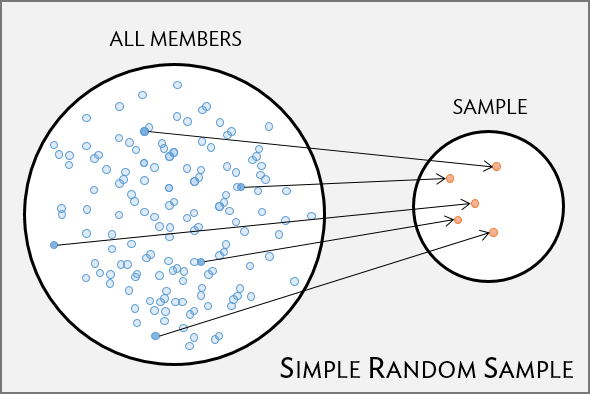
\includegraphics[scale=0.75]{003-sampleRandomHealthPlan.png}
\caption{Random sampling is the best way to ensure that a sample reflects a population. In a simple random sample, each member of a population has the same chance of being sampled. For example, suppose we want to estimate the proportion of Montrealers who do not have a family doctor. We should randomly sample from different households in Montreal.}
\end{figure}
%003-sampleConvenienceHealthPlan.png
%003-sampleNonResponseHealthPlan
\end{frame}




\begin{frame}{Selection bias}
	
	\begin{figure}
		\centering
		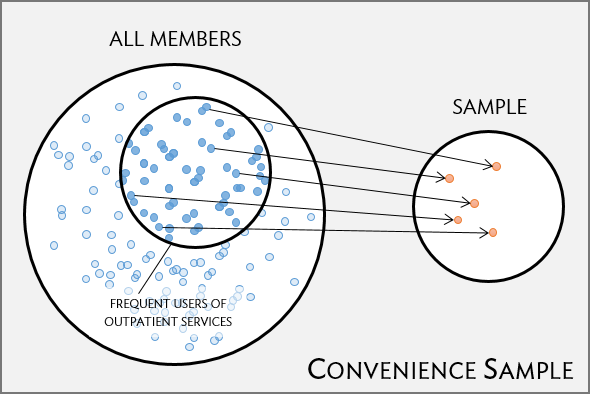
\includegraphics[scale=0.75]{003-sampleConvenienceHealthPlan.png}
		\caption{Instead of sampling from different households, we simply take all individuals from the same household.}
	\end{figure}
	%003-sampleConvenienceHealthPlan.png
	%003-sampleNonResponseHealthPlan
\end{frame}



\begin{frame}{The five ``W''s and 1 ``H''}
	\textbf{Data values, no matter what kind, are useless without their context.}
	\pause 
	
	\begin{itemize}
		\item \alert{Who:}  Describe the individuals who were sampled (aka observations, subjects, biological samples, participants, experimental units, cases).
		
		\item \alert{What:}  Determine what is being measured. The characteristics recorded about each individual are called \textbf{variables}.
		
		\pause
		
		\item \alert{Why:}  What was the purpose of the survey/experiment/study?
		
		\item \alert{When:}  When was the research conducted?
		
		\item \alert{Where:}  Where was the research conducted?
		
	\pause
		
		\item \alert{How:}  Describe how the survey/experiment/study was conducted. Simple random sample (SRS), volunteers, select population, non-representative sample ?
	\end{itemize}
	
\end{frame}



\section{Data basics}

\begin{frame}{Example: the \emph{FAMuSS} study}
	\protect\hypertarget{example-the-famuss-study}{}
	
\begin{itemize}
\item The Functional polymorphisms Associated with human Muscle Size and Strength study (FA-
MuSS) measured a variety of demographic, phenotypic, and genetic characteristics for about 1,300
participants\footnote{\tiny{Thompson PD, Moyna M, Seip, R, et al., 2004. Functional Polymorphisms Associated with Human Muscle Size and
		Strength. Medicine and Science in Sports and Exercise 36:1132 - 1139.}}\footnote[,2]{\tiny{see \emph{Harrington 1st edition}, Section 1.2.2, for more details}}. 
	
			\pause 
			
	\item One goal of the study---examine the association of demographic, physiological and genetic characteristics with muscle strength.
	
	\begin{itemize}
		\tightlist
		\item
		In simpler terms, study the ``sports gene'' \emph{ACTN3}.
	\end{itemize}
	
	
\end{itemize}
	
	
	
\end{frame}

\begin{frame}[fragile]{Four rows from \emph{FAMuSS} data matrix}
	\protect\hypertarget{four-rows-from-famuss-data-matrix}{}
	
	\captionsetup[table]{labelformat=empty}
	
	\scriptsize
	
	\normalsize
	
	\small
	
\begin{knitrout}\scriptsize
\definecolor{shadecolor}{rgb}{0.969, 0.969, 0.969}\color{fgcolor}\begin{kframe}
\begin{alltt}
\hlcom{# devtools::install_github("OI-Biostat/oi_biostat_data")}
\hlkwd{library}\hlstd{(oibiostat)}
\hlkwd{data}\hlstd{(famuss)}
\hlstd{famuss} \hlopt
  \hlstd{dplyr}\hlopt{::}\hlkwd{glimpse}\hlstd{()}
\end{alltt}
\begin{verbatim}
## Rows: 595
## Columns: 9
## $ ndrm.ch     <dbl> 40.0, 25.0, 40.0, 125.0, 40.0, 75.0, 100.0, 57.1, 33.3, 20~
## $ drm.ch      <dbl> 40.0, 0.0, 0.0, 0.0, 20.0, 0.0, 0.0, -14.3, 0.0, 0.0, 25.0~
## $ sex         <fct> Female, Male, Female, Female, Female, Female, Female, Fema~
## $ age         <int> 27, 36, 24, 40, 32, 24, 30, 28, 27, 30, 20, 23, 24, 34, 31~
## $ race        <fct> Caucasian, Caucasian, Caucasian, Caucasian, Caucasian, His~
## $ height      <dbl> 65.0, 71.7, 65.0, 68.0, 61.0, 62.2, 65.0, 68.0, 68.2, 62.2~
## $ weight      <dbl> 199, 189, 134, 171, 118, 120, 134, 162, 189, 120, 131, 108~
## $ actn3.r577x <fct> CC, CT, CT, CT, CC, CT, TT, CT, CC, CT, CT, CT, TT, CT, CC~
## $ bmi         <dbl> 33.112, 25.845, 22.296, 25.998, 22.293, 21.805, 22.296, 24~
\end{verbatim}
\end{kframe}
\end{knitrout}

	
	\normalsize
	
\end{frame}

\begin{frame}{\emph{FAMuSS} Variables and their descriptions}
	\protect\hypertarget{famuss-variables-and-their-descriptions}{}
	
	\begin{center}
		\begin{tabular}{ll}
			{\bf Variable} & {\bf Description} \\
\hline 
\texttt{ndrm.ch} & Percent change in strength in the non-dominant arm, \\
& comparing strength after to before training \\
\texttt{drm.ch} & Percent change in strength in a participant's dominant arm.\\
			\texttt{sex} & Sex of the participant \\
			\texttt{age} & Age in years   \\
			\texttt{race} & Recorded as African Am (African American),\\
			& Caucasian, Asian, Hispanic, Other \\
			\texttt{height} & Height in inches    \\
			\texttt{weight} & Weight in pounds  \\
			\texttt{actn3.r577x} & Genotype at the location r577x in the ACTN3 gene. \\
			\texttt{bmi} & The participant's body mass index 
		\end{tabular}
	\end{center}
	
\end{frame}

\begin{frame}{Types of Variables}
	\protect\hypertarget{types-of-variables}{}
	
	\textbf{Numerical variables} take on numerical values, such that
	numerical operations (sums, differences, etc.) are reasonable.
	
	\begin{itemize}
		\item
		Discrete: only take on integer values (e.g., \# of family members)
		\item
		Continuous: can take on any value within a specified range (e.g.,
		height)
	\end{itemize}
	
	\pause
	
	\textbf{Categorical variables} take on values that are names or labels;
	the possible values are called the variable's \emph{levels}.
	
	\begin{itemize}
		\tightlist
		\item
		Ordinal: exists some natural ordering of levels (e.g., education, likert scale)
		\item
		Nominal: no natural ordering of levels (e.g., gender)
	\end{itemize}
	
\end{frame}

\begin{frame}{Types of variables}
	\protect\hypertarget{types-of-variables-1}{}
	
	\begin{figure}
		\centering
		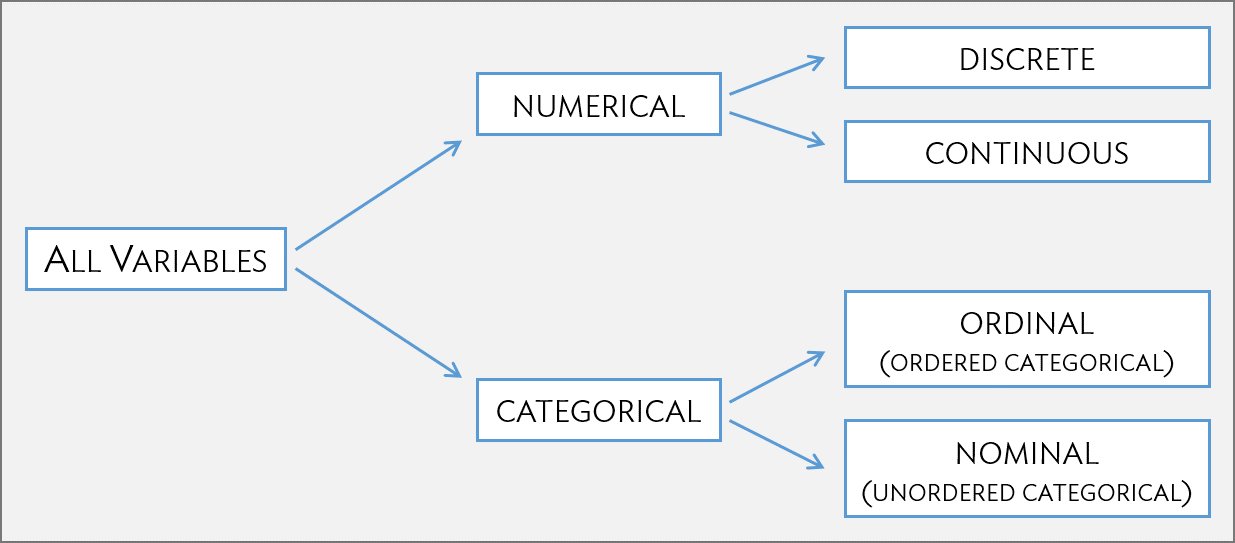
\includegraphics[scale=0.5]{figures/variableTypes.png}
		\caption{Types of variables}
	\end{figure}
	
\end{frame}



\begin{frame}{Exploring data with simple tools}
	\protect\hypertarget{exploring-data-with-simple-tools}{}
	
	\begin{itemize}
		\item Techniques for exploring and summarizing data differ for numerical
	versus categorical variables.
	
	\item Numerical and graphical summaries are useful for examining variables one
	at a time, but also for exploring the relationships between variables.
	\end{itemize}
	
\end{frame}


\section{Numerical data - single variable}\label{sec:numerical-data}

\begin{frame}{Distributions and summary measures}
	\protect\hypertarget{distributions-and-summary-measures}{}

\begin{itemize}
	\item  The collection of values for a numerical, continuous variable (e.g.,
	\texttt{weight}) is the \alert{distribution} for that variable.
	
	\pause 
	
\item 	Numerical and graphical summaries convey characteristics of a
	distribution without listing all the values.
	
\item Important characteristics include:
	
	\begin{itemize}
		\tightlist
		\item
		Center: where is the middle of the distribution?
		
		\begin{itemize}
			\tightlist
			\item
			Measures of center: mean, median
		\end{itemize}
	\pause 
	
		\item
		Spread: how similar or varied are the values to each other?
		
		\begin{itemize}
			\tightlist
			\item
			Measures of spread: standard deviation, interquartile range
		\end{itemize}
	\end{itemize}

\end{itemize}
	
\end{frame}



\begin{frame}[fragile]{Measures of center: mean}
The \alert{sample mean} of a variable is the sum of all observations divided by the number of observations:

$$\overline{y} = \frac{y_1+y_2+\cdots+y_n}{n}$$  
where $y_1, y_2, \ldots, y_n$ represent the $n$ observed values in a sample.

The mean weight in \texttt{famuss} is 155.65 pounds:

\begin{knitrout}\scriptsize
\definecolor{shadecolor}{rgb}{0.969, 0.969, 0.969}\color{fgcolor}\begin{kframe}
\begin{alltt}
\hlkwd{mean}\hlstd{(famuss}\hlopt{$}\hlstd{weight)}
\end{alltt}
\begin{verbatim}
## [1] 155.6479
\end{verbatim}
\end{kframe}
\end{knitrout}


\end{frame}


\begin{frame}[fragile]{Measures of center: median}
The \alert{median} is the value of the middle observation in a sample.  

If the number of observations is 

\begin{itemize}
	\item Odd, the median is the middle observation
	\item Even, the median is the average of the two middle observations
\end{itemize}

The median is the $50^{th}$ percentile; 50\% of observations lie below/above the median.

\begin{knitrout}\scriptsize
\definecolor{shadecolor}{rgb}{0.969, 0.969, 0.969}\color{fgcolor}\begin{kframe}
\begin{alltt}
\hlkwd{median}\hlstd{(famuss}\hlopt{$}\hlstd{weight)}
\end{alltt}
\begin{verbatim}
## [1] 150
\end{verbatim}
\begin{alltt}
\hlkwd{quantile}\hlstd{(famuss}\hlopt{$}\hlstd{weight,} \hlkwc{probs} \hlstd{=} \hlnum{0.50}\hlstd{)}
\end{alltt}
\begin{verbatim}
## 50% 
## 150
\end{verbatim}
\end{kframe}
\end{knitrout}

\end{frame}



\begin{frame}[fragile]{Measures of spread}
	\protect\hypertarget{measures-of-spread}{}
	
	The \emph{standard deviation} measures (approximately) the distance
	between a typical observation and the mean.
	
	\begin{itemize}
		\item
		An observation's \emph{deviation} is the distance between its value
		\(y\) and the sample mean \(\overline{y}\): \(y - \overline{y}\).
		\item
		The \emph{sample variance} \(s^2\) is the sum of squared deviations
		divided by the number of observations minus 1.
		\[s^2 = \frac{({y_1 - \overline{y})}^{2}+({y_2 - \overline{y})}^{2}+\cdots+({y_n - \overline{y})}^{2}}{n-1}, \]
		where \(y_1, y_2, \dots, y_n\) represent the \(n\) observed values.
		\item
		The \emph{standard deviation} \(s\) is the square root of the
		variance.
		\[s = \sqrt{\frac{({y_1 - \overline{y})}^{2}+({y_2 - \overline{y})}^{2}+\cdots+({y_n - \overline{y})}^{2}}{n-1}}\]
	\end{itemize}

\begin{knitrout}\scriptsize
\definecolor{shadecolor}{rgb}{0.969, 0.969, 0.969}\color{fgcolor}\begin{kframe}
\begin{alltt}
\hlkwd{sd}\hlstd{(famuss}\hlopt{$}\hlstd{weight)}
\end{alltt}
\begin{verbatim}
## [1] 34.58999
\end{verbatim}
\end{kframe}
\end{knitrout}
	
\end{frame}

\begin{frame}[fragile]{Measures of Spread: Percentiles/Quartiles}
	\protect\hypertarget{measures-of-spread-percentilesquartiles}{}
	
	The \(p^{th}\) percentile is the observation such that \(p\%\) of the
	remaining observations fall below this observation.
	
	\begin{itemize}
		\tightlist
		\item
		The \emph{first quartile (\(Q_1\))} is the \(25^{th}\) percentile.
		\item
		The \emph{second quartile (\(Q_2\))}, i.e., the median, is the
		\(50^{th}\) percentile.
		\item
		The \emph{third quartile (\(Q_3\))} is the \(75^{th}\) percentile.
	\end{itemize}
	
	The \emph{interquartile range (IQR)} is the distance between the third
	and first quartiles. \[IQR = Q_3 - Q_1 \]
	
	\footnotesize
	
	\scriptsize
	
\begin{knitrout}\scriptsize
\definecolor{shadecolor}{rgb}{0.969, 0.969, 0.969}\color{fgcolor}\begin{kframe}
\begin{alltt}
\hlkwd{IQR}\hlstd{(famuss}\hlopt{$}\hlstd{weight)}
\end{alltt}
\begin{verbatim}
## [1] 42
\end{verbatim}
\begin{alltt}
\hlkwd{diff}\hlstd{(}\hlkwd{quantile}\hlstd{(famuss}\hlopt{$}\hlstd{weight,} \hlkwc{probs} \hlstd{=} \hlkwd{c}\hlstd{(}\hlnum{0.25}\hlstd{,} \hlnum{0.75}\hlstd{)))}
\end{alltt}
\begin{verbatim}
## 75% 
##  42
\end{verbatim}
\end{kframe}
\end{knitrout}

					
	\normalsize
					
\end{frame}


\begin{frame}{Robust estimates}
	\protect\hypertarget{robust-estimates}{}
	
\begin{itemize}
	\item 	The median and IQR are called \alert{robust estimates} because they are
	less likely to be affected by extreme values than the mean and standard
	deviation.
	
	\item For distributions containing extreme observations, the median and IQR
	provide a more accurate sense of center and spread.
\end{itemize}
	
\end{frame}

\begin{frame}[fragile]{Histograms}
	\protect\hypertarget{histograms}{}
	
	\scriptsize
	
\begin{knitrout}\scriptsize
\definecolor{shadecolor}{rgb}{0.969, 0.969, 0.969}\color{fgcolor}\begin{kframe}
\begin{alltt}
\hlkwd{hist}\hlstd{(famuss}\hlopt{$}\hlstd{weight,} \hlkwc{breaks} \hlstd{=} \hlnum{30}\hlstd{,} \hlkwc{col} \hlstd{=} \hlstr{'lightblue'}\hlstd{)}
\hlkwd{abline}\hlstd{(}\hlkwc{v} \hlstd{=} \hlkwd{mean}\hlstd{(famuss}\hlopt{$}\hlstd{weight),} \hlkwc{lwd} \hlstd{=} \hlnum{3}\hlstd{,} \hlkwc{col} \hlstd{=} \hlstr{"red"}\hlstd{)}
\hlkwd{abline}\hlstd{(}\hlkwc{v} \hlstd{=} \hlkwd{median}\hlstd{(famuss}\hlopt{$}\hlstd{weight),} \hlkwc{lwd} \hlstd{=} \hlnum{3}\hlstd{,} \hlkwc{col} \hlstd{=} \hlstr{"blue"}\hlstd{)}
\hlkwd{legend}\hlstd{(}\hlstr{"topright"}\hlstd{,} \hlkwc{legend} \hlstd{=} \hlkwd{c}\hlstd{(}\hlstr{"mean"}\hlstd{,}\hlstr{"median"}\hlstd{),} \hlkwc{col} \hlstd{=} \hlkwd{c}\hlstd{(}\hlstr{"red"}\hlstd{,}\hlstr{"blue"}\hlstd{),} \hlkwc{lwd} \hlstd{=} \hlnum{3}\hlstd{)}
\end{alltt}
\end{kframe}

{\centering 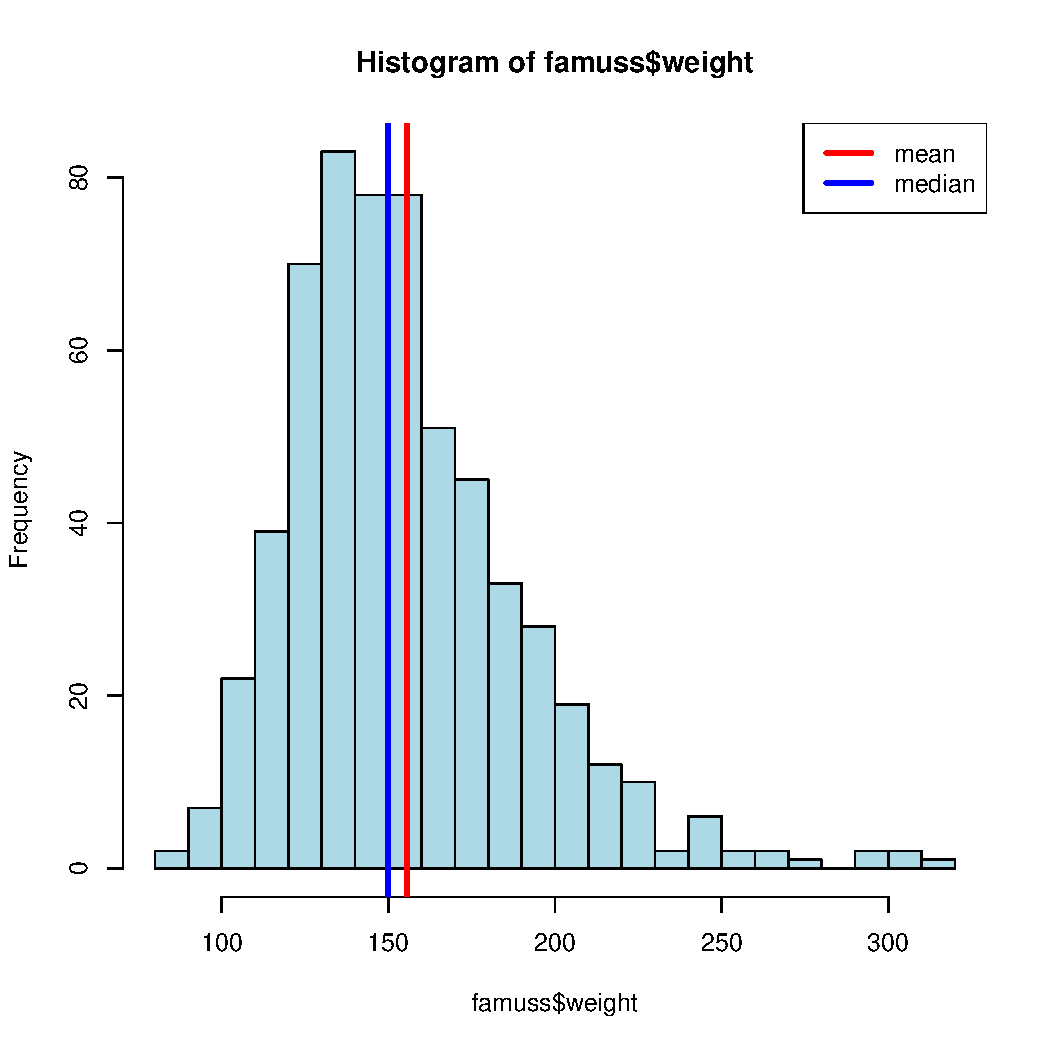
\includegraphics[width=0.6\linewidth]{figure/hist_weight-1-1} 

}


\end{knitrout}

\normalsize
			
\end{frame}

\begin{frame}[fragile]{Histograms}
	\protect\hypertarget{histograms}{}
	
	\scriptsize
	
\begin{knitrout}\scriptsize
\definecolor{shadecolor}{rgb}{0.969, 0.969, 0.969}\color{fgcolor}\begin{kframe}
\begin{alltt}
\hlkwd{hist}\hlstd{(famuss}\hlopt{$}\hlstd{weight,} \hlkwc{breaks} \hlstd{=} \hlnum{5}\hlstd{,} \hlkwc{col} \hlstd{=} \hlstr{'lightblue'}\hlstd{)}
\hlkwd{abline}\hlstd{(}\hlkwc{v} \hlstd{=} \hlkwd{mean}\hlstd{(famuss}\hlopt{$}\hlstd{weight),} \hlkwc{lwd} \hlstd{=} \hlnum{3}\hlstd{,} \hlkwc{col} \hlstd{=} \hlstr{"red"}\hlstd{)}
\hlkwd{abline}\hlstd{(}\hlkwc{v} \hlstd{=} \hlkwd{median}\hlstd{(famuss}\hlopt{$}\hlstd{weight),} \hlkwc{lwd} \hlstd{=} \hlnum{3}\hlstd{,} \hlkwc{col} \hlstd{=} \hlstr{"blue"}\hlstd{)}
\hlkwd{legend}\hlstd{(}\hlstr{"topright"}\hlstd{,} \hlkwc{legend} \hlstd{=} \hlkwd{c}\hlstd{(}\hlstr{"mean"}\hlstd{,}\hlstr{"median"}\hlstd{),} \hlkwc{col} \hlstd{=} \hlkwd{c}\hlstd{(}\hlstr{"red"}\hlstd{,}\hlstr{"blue"}\hlstd{),} \hlkwc{lwd} \hlstd{=} \hlnum{3}\hlstd{)}
\end{alltt}
\end{kframe}

{\centering 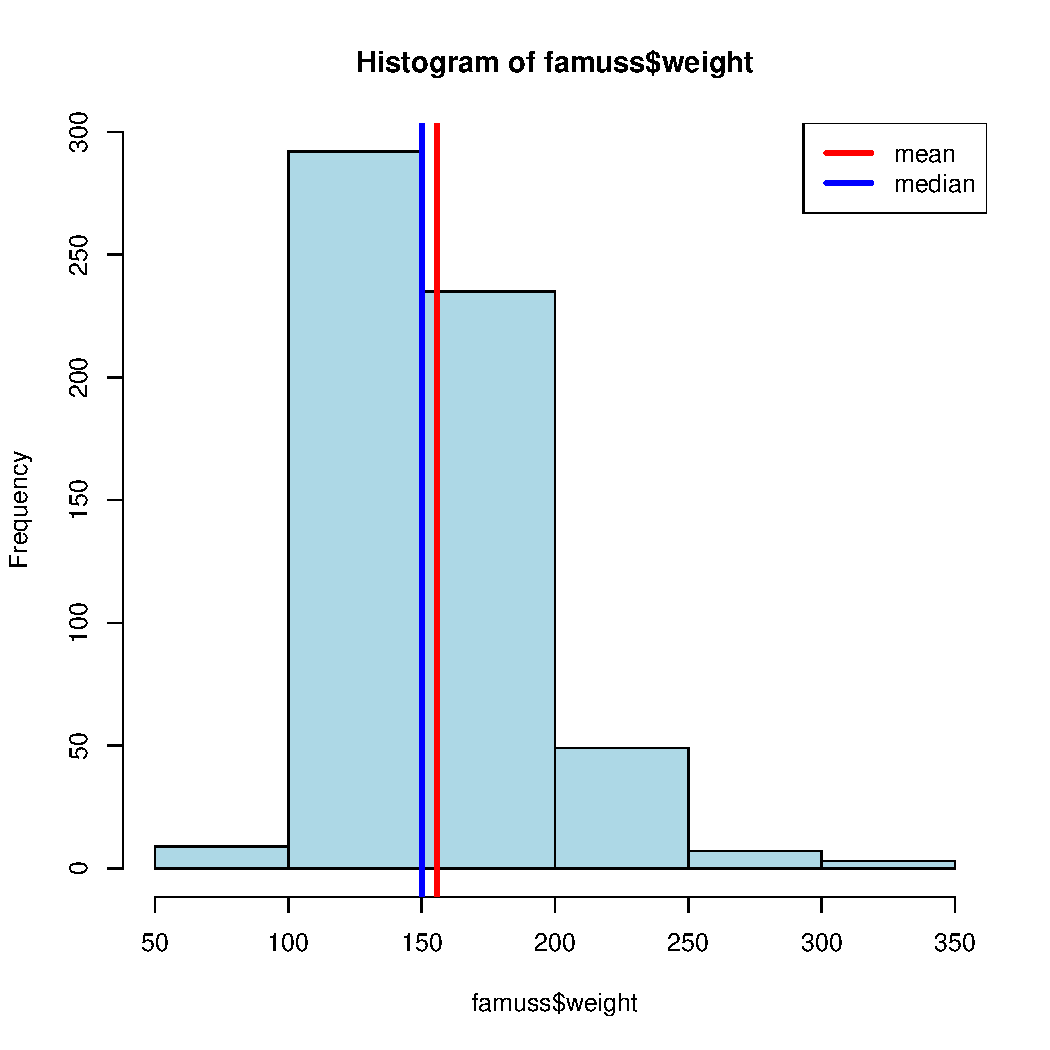
\includegraphics[width=0.6\linewidth]{figure/hist_weight-2-1} 

}


\end{knitrout}
	
	\normalsize
	
\end{frame}



\begin{frame}[fragile]{Density plots}

	
	\scriptsize
	
\begin{knitrout}\scriptsize
\definecolor{shadecolor}{rgb}{0.969, 0.969, 0.969}\color{fgcolor}\begin{kframe}
\begin{alltt}
\hlkwd{hist}\hlstd{(famuss}\hlopt{$}\hlstd{weight,} \hlkwc{breaks} \hlstd{=} \hlnum{30}\hlstd{,} \hlkwc{col} \hlstd{=} \hlstr{'lightblue'}\hlstd{,} \hlkwc{probability} \hlstd{=} \hlnum{TRUE}\hlstd{)}
\hlstd{openintro}\hlopt{::}\hlkwd{densityPlot}\hlstd{(famuss}\hlopt{$}\hlstd{weight,} \hlkwc{add} \hlstd{=} \hlnum{TRUE}\hlstd{,} \hlkwc{lwd} \hlstd{=} \hlnum{5}\hlstd{)}
\hlkwd{abline}\hlstd{(}\hlkwc{v} \hlstd{=} \hlkwd{mean}\hlstd{(famuss}\hlopt{$}\hlstd{weight),} \hlkwc{lwd} \hlstd{=} \hlnum{3}\hlstd{,} \hlkwc{col} \hlstd{=} \hlstr{"red"}\hlstd{)}
\hlkwd{abline}\hlstd{(}\hlkwc{v} \hlstd{=} \hlkwd{median}\hlstd{(famuss}\hlopt{$}\hlstd{weight),} \hlkwc{lwd} \hlstd{=} \hlnum{3}\hlstd{,} \hlkwc{col} \hlstd{=} \hlstr{"blue"}\hlstd{)}
\hlkwd{legend}\hlstd{(}\hlstr{"topright"}\hlstd{,} \hlkwc{legend} \hlstd{=} \hlkwd{c}\hlstd{(}\hlstr{"mean"}\hlstd{,}\hlstr{"median"}\hlstd{,}\hlstr{"density"}\hlstd{),}
       \hlkwc{col} \hlstd{=} \hlkwd{c}\hlstd{(}\hlstr{"red"}\hlstd{,}\hlstr{"blue"}\hlstd{,}\hlstr{"black"}\hlstd{),} \hlkwc{lwd} \hlstd{=} \hlnum{3}\hlstd{)}
\end{alltt}
\end{kframe}

{\centering 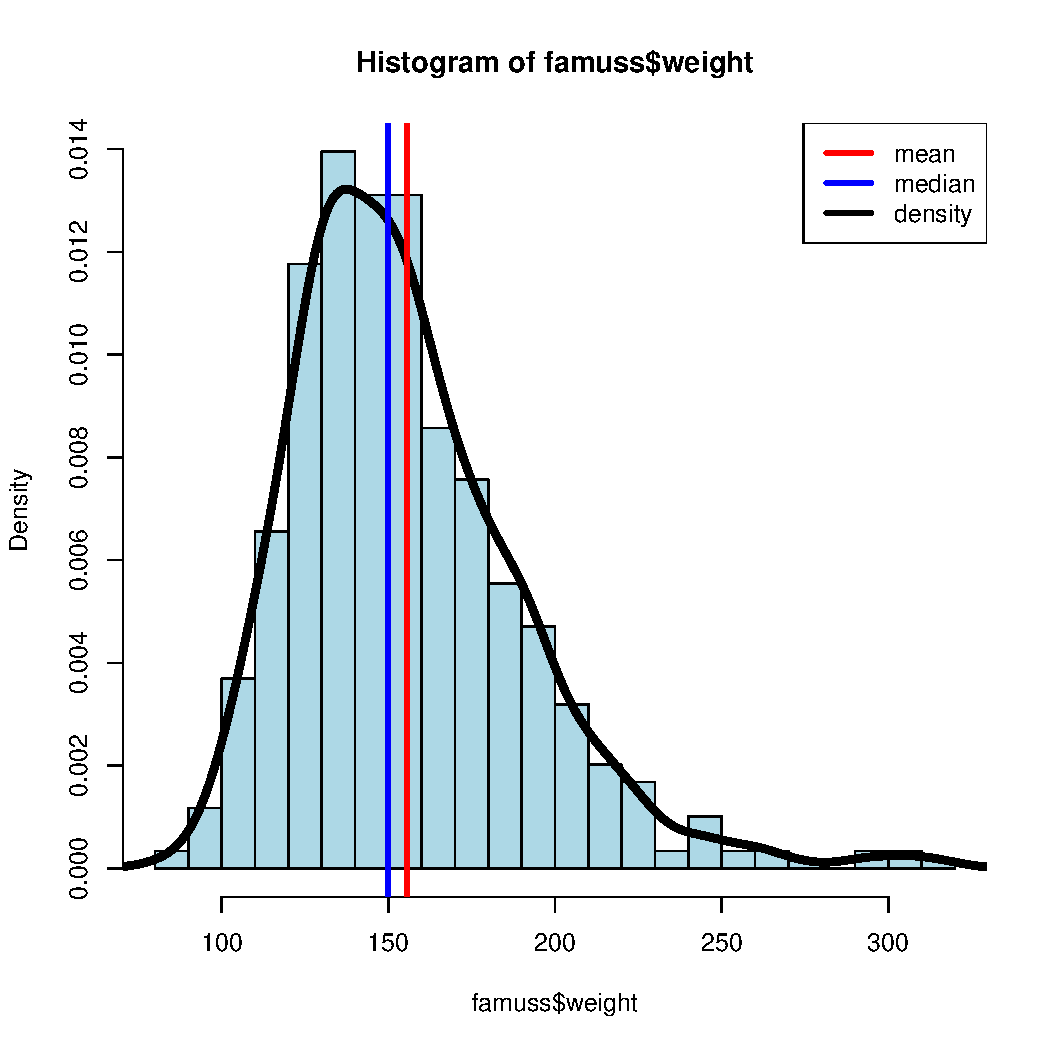
\includegraphics[width=0.6\linewidth]{figure/hist_weight-3-1} 

}


\end{knitrout}
	
	\normalsize
	
\end{frame}


		
\begin{frame}{Histograms \dots}
			\protect\hypertarget{histograms-1}{}

\begin{itemize}
\item Histograms show important features of the shape of a distribution:
			
			\begin{itemize}
				\item
				Symmetry, or lack of it (skew)
				\item
				Minimum and maximum values
				\item
				Regions of high frequency (modes)
			\end{itemize}
	\pause		
		\item 	Histograms not so good for:
			
			\begin{itemize}
				\item
				Displaying median, quartiles
				\item
				Showing subtle skewing
				\item
				Identifying extreme values
			\end{itemize}
		
		\pause
		\item Remember that histograms are sensitive to the number of bins!

\end{itemize}			
			
\end{frame}




		
\begin{frame}[fragile]{Boxplot for \texttt{weight}}
			\protect\hypertarget{oi-biostat-figure-1.20-frog-data}{}
			
\begin{knitrout}\tiny
\definecolor{shadecolor}{rgb}{0.969, 0.969, 0.969}\color{fgcolor}

{\centering 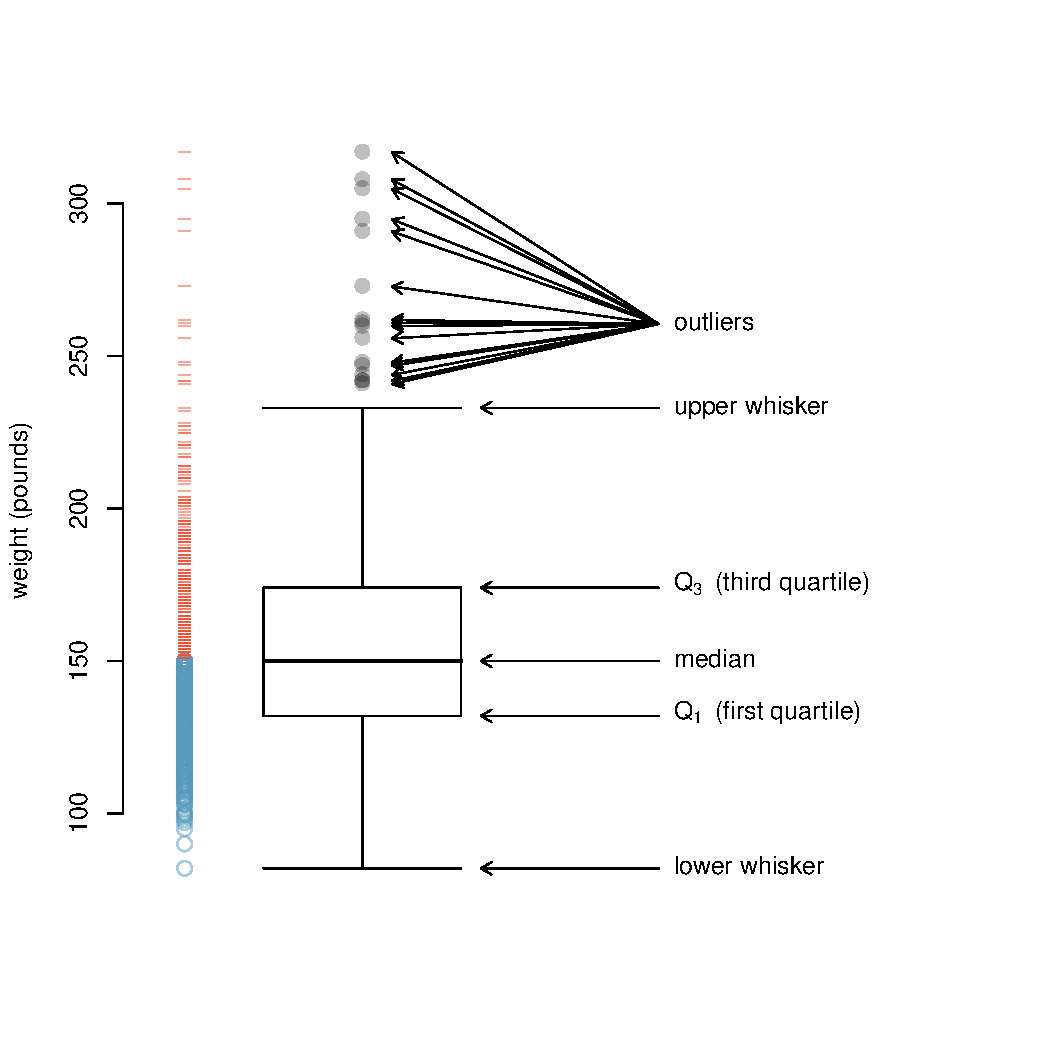
\includegraphics[width=0.85\linewidth]{figure/boxplot-1} 

}


\end{knitrout}
			
\end{frame}
		

\begin{frame}{Boxplots}
			\protect\hypertarget{boxplots}{}
			
			A boxplot indicates the positions of the first, second, and third
			quartiles of a distribution in addition to potential \textbf{outliers},
			observations that are far from the center of a distribution.
			
			\begin{itemize}
				\item
				Large outliers: values \textgreater{} \(Q_3 + (1.5\times IQR)\)
				\item
				Small outliers: values \textless{} \(Q_1 - (1.5 \times IQR)\)
			\end{itemize}
			
			On a boxplot\ldots{}
			
			\begin{itemize}
				\item
				The rectangle extends from the first quartile to the third quartile,
				with a line at the second quartile (median).
				\item
				Whiskers capture data between \(Q_1 - (1.5 \times IQR)\) and
				\(Q_3 + (1.5\times IQR)\) ; whiskers must end at data points.
				\item
				Potential outliers shown with dots.
			\end{itemize}
			
\end{frame}


\begin{frame}[fragile]{Boxplots vs. Violin plots}
	
\begin{knitrout}\scriptsize
\definecolor{shadecolor}{rgb}{0.969, 0.969, 0.969}\color{fgcolor}\begin{kframe}
\begin{alltt}
\hlstd{p1} \hlkwb{<-} \hlkwd{ggplot}\hlstd{(}\hlkwc{data} \hlstd{= famuss,} \hlkwc{mapping} \hlstd{=} \hlkwd{aes}\hlstd{(}\hlkwc{x} \hlstd{=} \hlstr{"all"}\hlstd{,} \hlkwc{y} \hlstd{= weight))} \hlopt{+} \hlkwd{theme_minimal}\hlstd{()}
\hlstd{p1} \hlopt{+} \hlkwd{geom_boxplot}\hlstd{()}
\hlstd{p1} \hlopt{+} \hlkwd{geom_violin}\hlstd{()}
\end{alltt}
\end{kframe}

{\centering 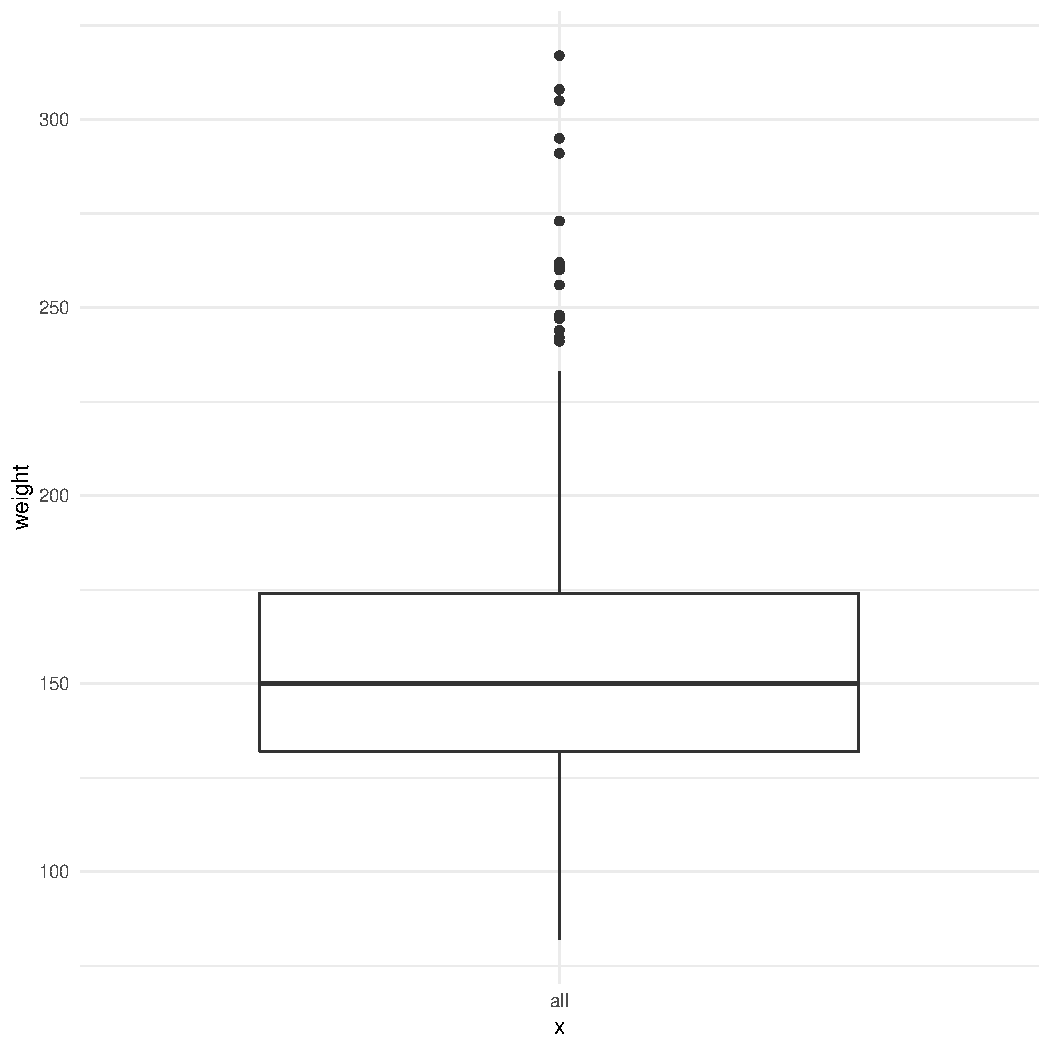
\includegraphics[width=0.45\linewidth]{figure/unnamed-chunk-2-1} 
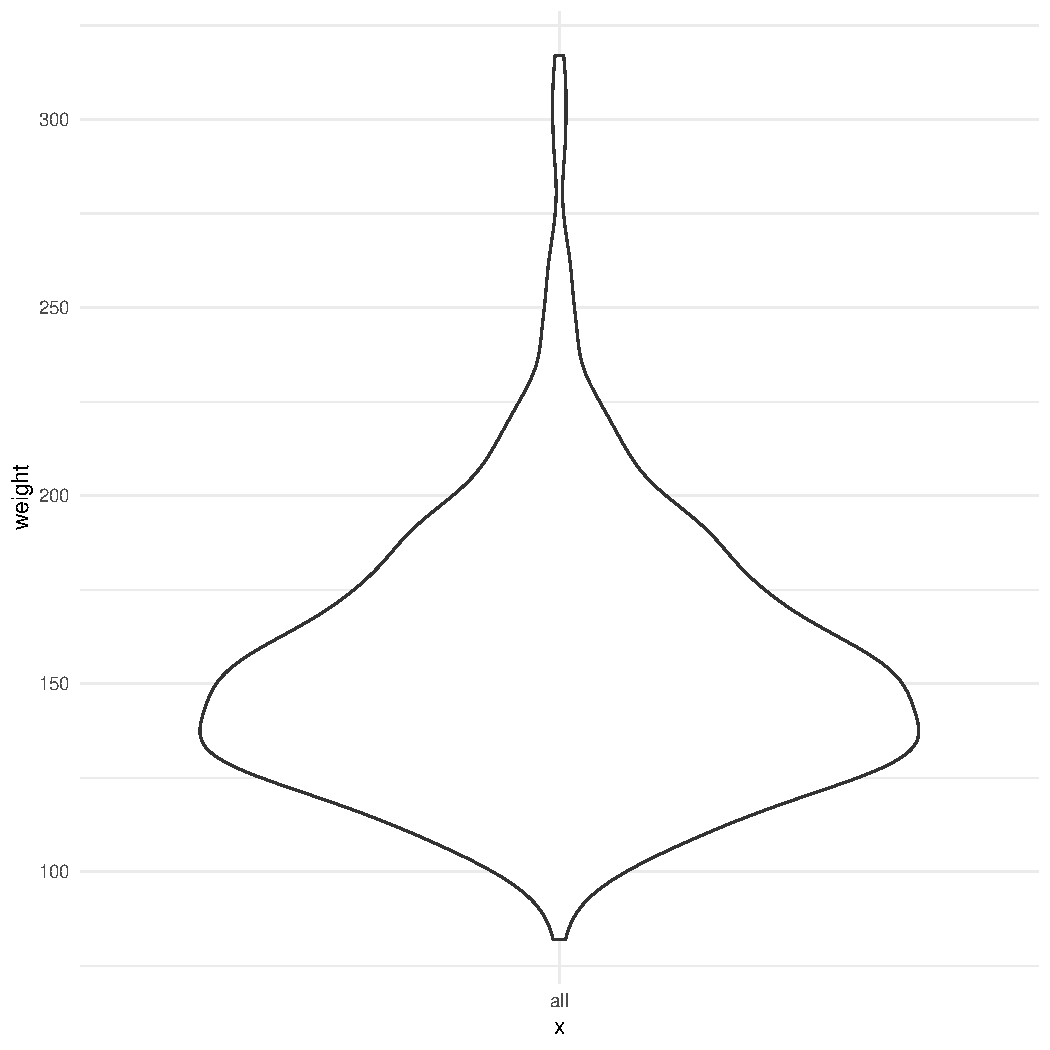
\includegraphics[width=0.45\linewidth]{figure/unnamed-chunk-2-2} 

}


\end{knitrout}
	
\end{frame}

		
		\hypertarget{categorical-data}{%
	\section{Categorical data - single variable}\label{categorical-data}}
		
\begin{frame}[fragile]{Tables}
			\protect\hypertarget{tables}{}
			
			A table for a single variable, a \emph{frequency table} or \emph{one-way
				table}, summarizes the distribution of observations among categories.
			
			Based on the table, describe the distribution of genotype at the
			location \emph{actn3.r577x} among the study participants.
			
			\small
			
			\scriptsize

\begin{knitrout}\scriptsize
\definecolor{shadecolor}{rgb}{0.969, 0.969, 0.969}\color{fgcolor}\begin{kframe}
\begin{alltt}
\hlkwd{table}\hlstd{(famuss}\hlopt{$}\hlstd{actn3.r577x)}
\end{alltt}
\begin{verbatim}
## 
##  CC  CT  TT 
## 173 261 161
\end{verbatim}
\end{kframe}
\end{knitrout}

		
		\normalsize
					
\end{frame}
				

\begin{frame}[fragile]{Bar plots for categorical data}
					\protect\hypertarget{bar-plots-for-categorical-data}{}
					
					A bar plot is a common way to display a single categorical variable.
					
					\small
					
					\scriptsize
					
\begin{knitrout}\scriptsize
\definecolor{shadecolor}{rgb}{0.969, 0.969, 0.969}\color{fgcolor}\begin{kframe}
\begin{alltt}
\hlstd{graphics}\hlopt{::}\hlkwd{barplot}\hlstd{(}\hlkwd{table}\hlstd{(famuss}\hlopt{$}\hlstd{actn3.r577x))}
\hlstd{sjPlot}\hlopt{::}\hlkwd{plot_frq}\hlstd{(famuss}\hlopt{$}\hlstd{actn3.r577x)}
\end{alltt}
\end{kframe}

{\centering 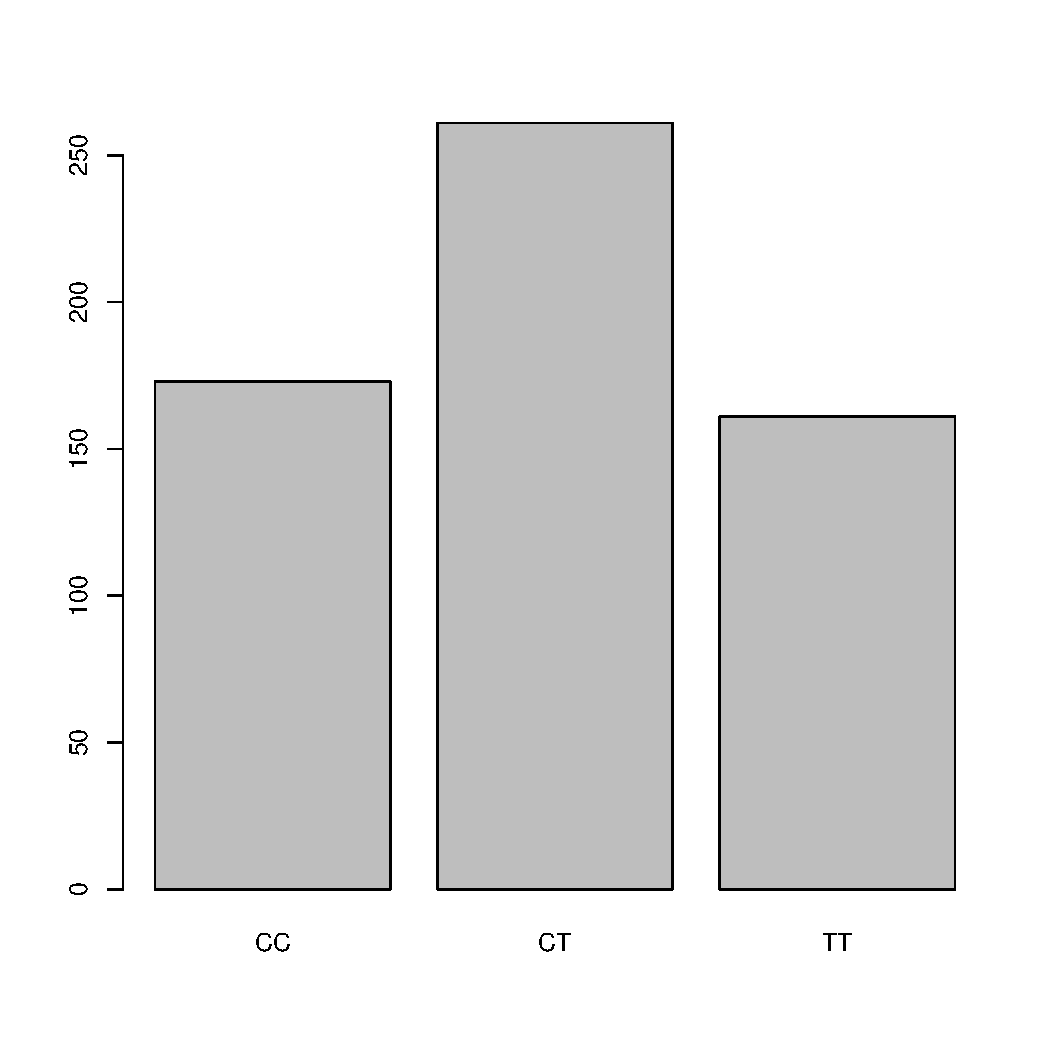
\includegraphics[width=0.45\linewidth]{figure/table-2-1} 
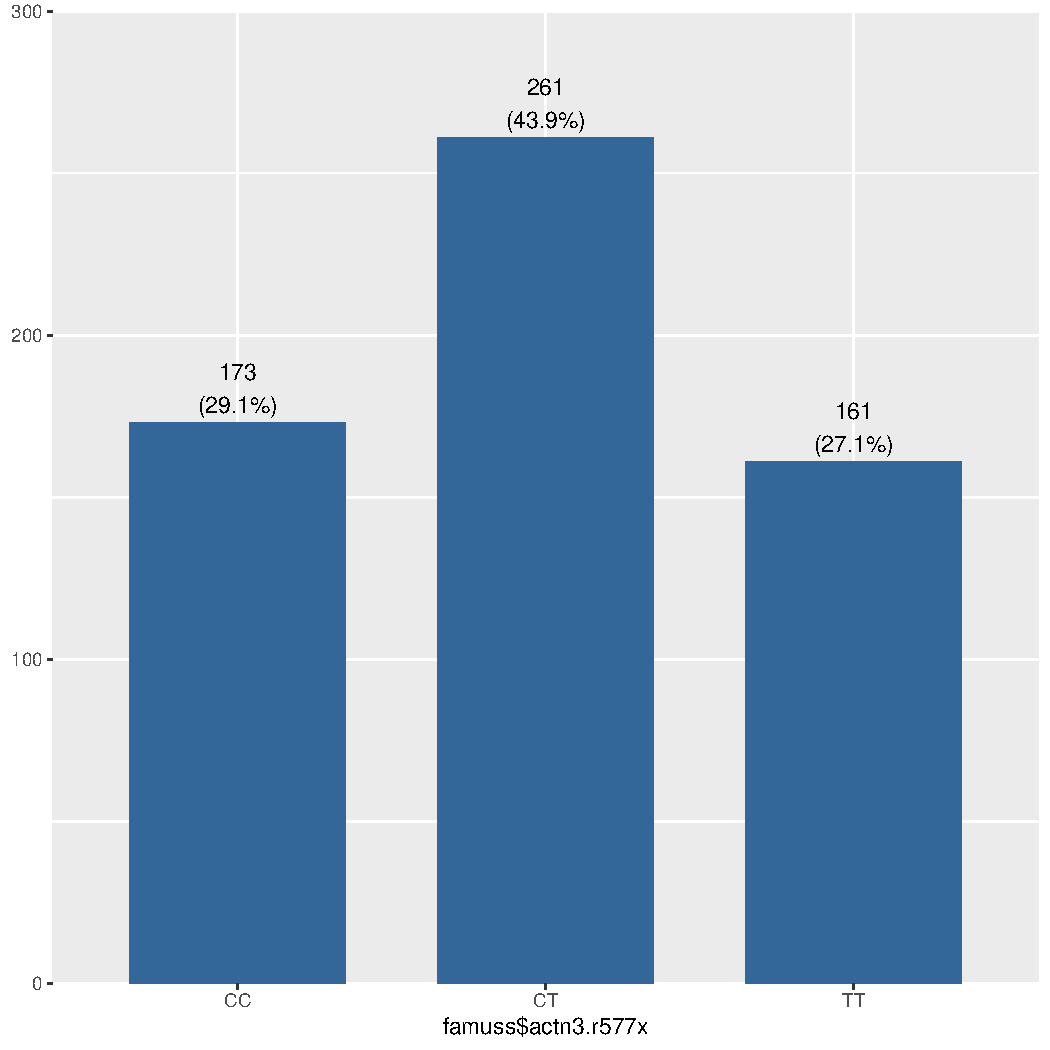
\includegraphics[width=0.45\linewidth]{figure/table-2-2} 

}


\end{knitrout}
							\normalsize
							
\end{frame}
						


\end{document}	
	
	\hypertarget{relationships-between-two-variables}{%
	\section{Relationships between two variables}\label{relationships-between-two-variables}}
						
\begin{frame}{Summarizing relationships between two variables}
							\protect\hypertarget{summarizing-relationships-between-two-variables}{}
							
							Approaches for summarizing relationships between two variables vary
							depending on variable types\ldots{}
							
							\begin{itemize}
								\item
								Two numerical variables
								\item
								Two categorical variables
								\item
								One numerical variable and one categorical variable
							\end{itemize}
							
\end{frame}
						
						\begin{frame}{Two numerical variables}
							\protect\hypertarget{two-numerical-variables}{}
							
							Two variables \(x\) and \(y\) are
							
							\begin{itemize}
								\item
								\emph{positively associated} if \(y\) increases as \(x\) increases.
								\item
								\emph{negatively associated} if \(y\) decreases as \(x\) increases.
							\end{itemize}
							
							Height and weight are positively associated.
							
						\end{frame}
						
						\begin{frame}[fragile]{Two numerical variables \dots}
							\protect\hypertarget{two-numerical-variables-1}{}
							
							\small
							
							\scriptsize
							
							
\begin{knitrout}\scriptsize
\definecolor{shadecolor}{rgb}{0.969, 0.969, 0.969}\color{fgcolor}\begin{kframe}
\begin{alltt}
\hlkwd{plot}\hlstd{(famuss}\hlopt{$}\hlstd{height, famuss}\hlopt{$}\hlstd{weight,}
     \hlkwc{xlab} \hlstd{=} \hlstr{"Height (in)"}\hlstd{,} \hlkwc{ylab} \hlstd{=} \hlstr{"Weight (lb)"}\hlstd{,} \hlkwc{cex} \hlstd{=} \hlnum{0.8}\hlstd{)}

\hlkwd{ggplot}\hlstd{(}\hlkwc{data} \hlstd{= famuss,} \hlkwc{mapping} \hlstd{=} \hlkwd{aes}\hlstd{(}\hlkwc{x} \hlstd{= height,} \hlkwc{y} \hlstd{= weight))} \hlopt{+}
   \hlkwd{geom_point}\hlstd{(}\hlkwc{size} \hlstd{=} \hlnum{0.8}\hlstd{,} \hlkwc{pch} \hlstd{=} \hlnum{21}\hlstd{)}
\end{alltt}
\end{kframe}

{\centering 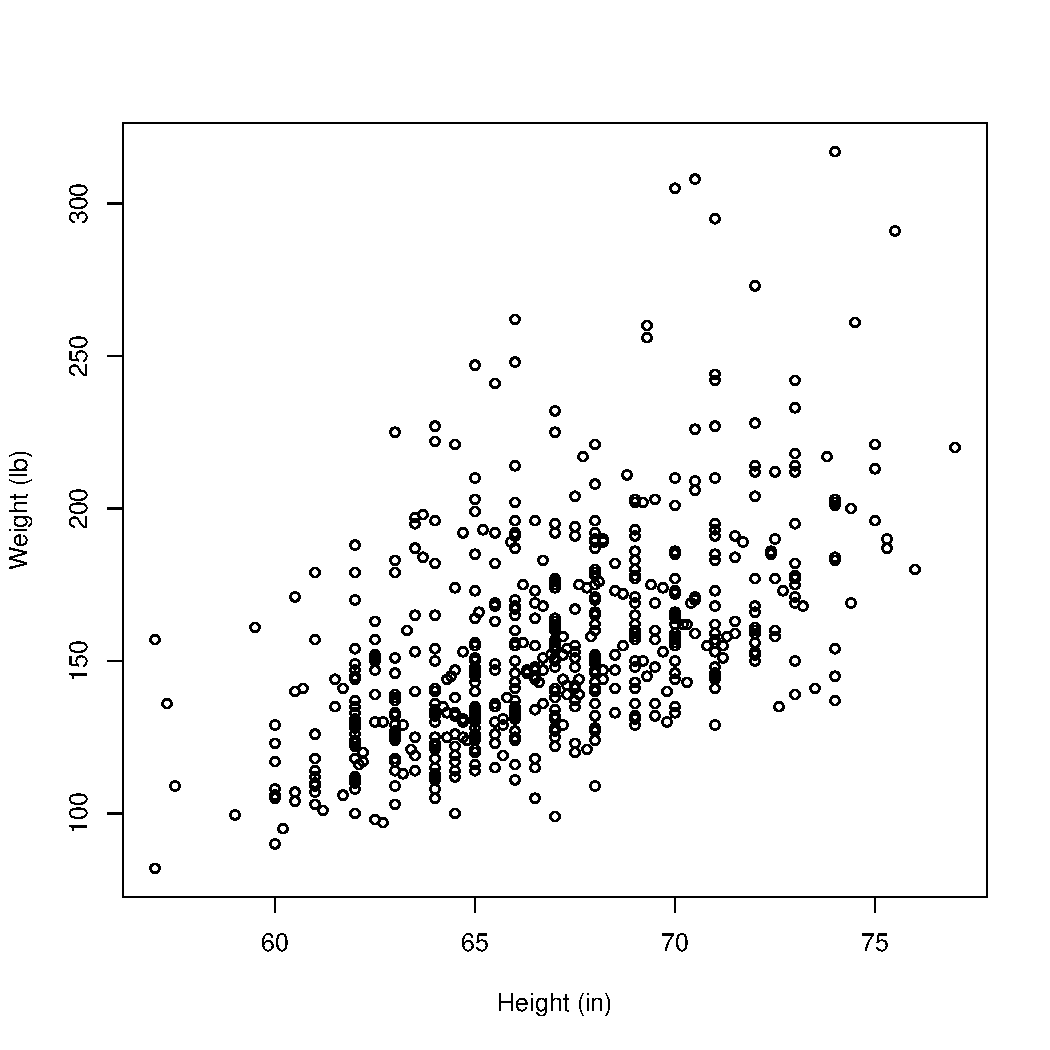
\includegraphics[width=0.45\linewidth]{figure/numerical-1} 
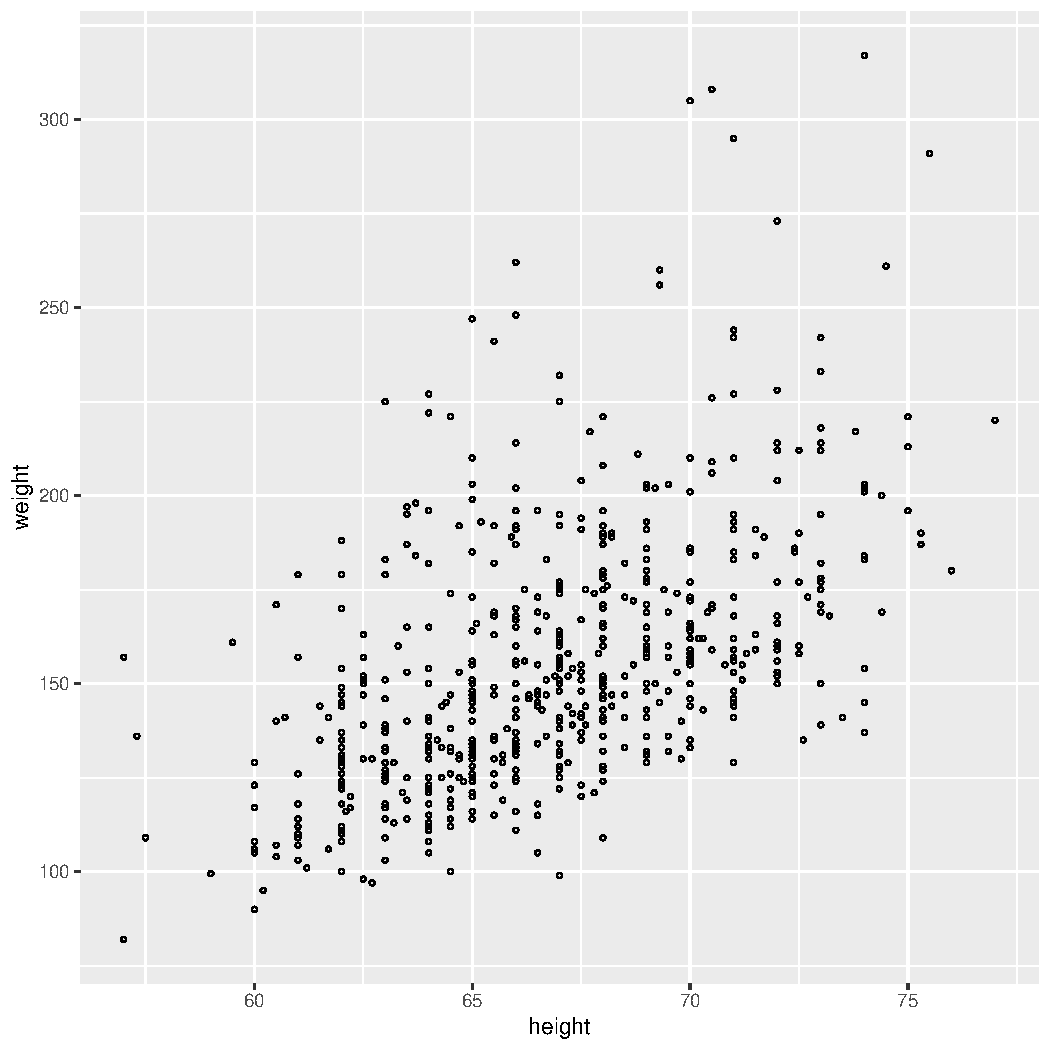
\includegraphics[width=0.45\linewidth]{figure/numerical-2} 

}


\end{knitrout}
							
	\normalsize
				
\end{frame}

						
\begin{frame}[fragile]{Two numerical variables \dots}
							\protect\hypertarget{two-numerical-variables-2}{}
							
					Correlation is a numerical summary that measures the strength of a
							linear relationship between two variables.
							
							\begin{itemize}
								\item
								Introduced in \emph{OI Biostat} Section 1.6.1; details in Ch. 6.
								\item
								The correlation coefficient \(r\) takes on values between -1 and 1.
								\item
								The closer \(r\) is to \(\pm 1\), the stronger the linear association.
							\end{itemize}
							
							\scriptsize
							
\begin{knitrout}\tiny
\definecolor{shadecolor}{rgb}{0.969, 0.969, 0.969}\color{fgcolor}\begin{kframe}
\begin{alltt}
\hlkwd{cor}\hlstd{(famuss}\hlopt{$}\hlstd{height, famuss}\hlopt{$}\hlstd{weight)}
\end{alltt}
\begin{verbatim}
## [1] 0.5308787
\end{verbatim}
\begin{alltt}
\hlkwd{summary}\hlstd{(}\hlkwd{lm}\hlstd{(height} \hlopt{~} \hlstd{weight,} \hlkwc{data} \hlstd{= famuss))}
\end{alltt}
\begin{verbatim}
## Coefficients:
##              Estimate Std. Error t value Pr(>|t|)    
## (Intercept) 58.295213   0.573200  101.70   <2e-16 ***
## weight       0.054843   0.003595   15.26   <2e-16 ***
## ---
## Signif. codes:  0 '***' 0.001 '**' 0.01 '*' 0.05 '.' 0.1 ' ' 1
## 
## Residual standard error: 3.031 on 593 degrees of freedom
## Multiple R-squared: 0.2818,	Adjusted R-squared: 0.2806 
## F-statistic: 232.7 on 1 and 593 DF,  p-value: < 2.2e-16
\end{verbatim}
\end{kframe}
\end{knitrout}
							
						
							\normalsize
							
						\end{frame}
						
						\begin{frame}[fragile]{Two categorical variables}
							\protect\hypertarget{two-categorical-variables}{}
							
							A contingency table summarizes data for two categorical variables.
							
							\scriptsize
							
\begin{knitrout}\scriptsize
\definecolor{shadecolor}{rgb}{0.969, 0.969, 0.969}\color{fgcolor}\begin{kframe}
\begin{alltt}
\hlkwd{addmargins}\hlstd{(}\hlkwd{table}\hlstd{(famuss}\hlopt{$}\hlstd{race, famuss}\hlopt{$}\hlstd{actn3.r577x))}
\end{alltt}
\begin{verbatim}
##             
##               CC  CT  TT Sum
##   African Am  16   6   5  27
##   Asian       21  18  16  55
##   Caucasian  125 216 126 467
##   Hispanic     4  10   9  23
##   Other        7  11   5  23
##   Sum        173 261 161 595
\end{verbatim}
\end{kframe}
\end{knitrout}
							
						
							
							\normalsize
							
						\end{frame}
						
						\begin{frame}[fragile]{Two categorical variables \dots}
							\protect\hypertarget{two-categorical-variables-1}{}
							
							\scriptsize
							
							\scriptsize
							
\begin{knitrout}\scriptsize
\definecolor{shadecolor}{rgb}{0.969, 0.969, 0.969}\color{fgcolor}\begin{kframe}
\begin{alltt}
\hlcom{#row proportions}
\hlkwd{addmargins}\hlstd{(}\hlkwd{prop.table}\hlstd{(}\hlkwd{table}\hlstd{(famuss}\hlopt{$}\hlstd{race, famuss}\hlopt{$}\hlstd{actn3.r577x),} \hlnum{1}\hlstd{))}
\end{alltt}
\begin{verbatim}
##             
##                     CC        CT        TT       Sum
##   African Am 0.5925926 0.2222222 0.1851852 1.0000000
##   Asian      0.3818182 0.3272727 0.2909091 1.0000000
##   Caucasian  0.2676660 0.4625268 0.2698073 1.0000000
##   Hispanic   0.1739130 0.4347826 0.3913043 1.0000000
##   Other      0.3043478 0.4782609 0.2173913 1.0000000
##   Sum        1.7203376 1.9250652 1.3545972 5.0000000
\end{verbatim}
\end{kframe}
\end{knitrout}
							
\begin{knitrout}\scriptsize
\definecolor{shadecolor}{rgb}{0.969, 0.969, 0.969}\color{fgcolor}\begin{kframe}
\begin{alltt}
\hlcom{#column proportions}
\hlkwd{addmargins}\hlstd{(}\hlkwd{prop.table}\hlstd{(}\hlkwd{table}\hlstd{(famuss}\hlopt{$}\hlstd{race, famuss}\hlopt{$}\hlstd{actn3.r577x),} \hlnum{2}\hlstd{))}
\end{alltt}
\begin{verbatim}
##             
##                      CC         CT         TT        Sum
##   African Am 0.09248555 0.02298851 0.03105590 0.14652996
##   Asian      0.12138728 0.06896552 0.09937888 0.28973168
##   Caucasian  0.72254335 0.82758621 0.78260870 2.33273826
##   Hispanic   0.02312139 0.03831418 0.05590062 0.11733618
##   Other      0.04046243 0.04214559 0.03105590 0.11366392
##   Sum        1.00000000 1.00000000 1.00000000 3.00000000
\end{verbatim}
\end{kframe}
\end{knitrout}
							
							
							\normalsize
							
						\end{frame}
						
						\begin{frame}{Two categorical variables \dots}
							\protect\hypertarget{two-categorical-variables-2}{}
							
							\begin{figure}
								\centering
								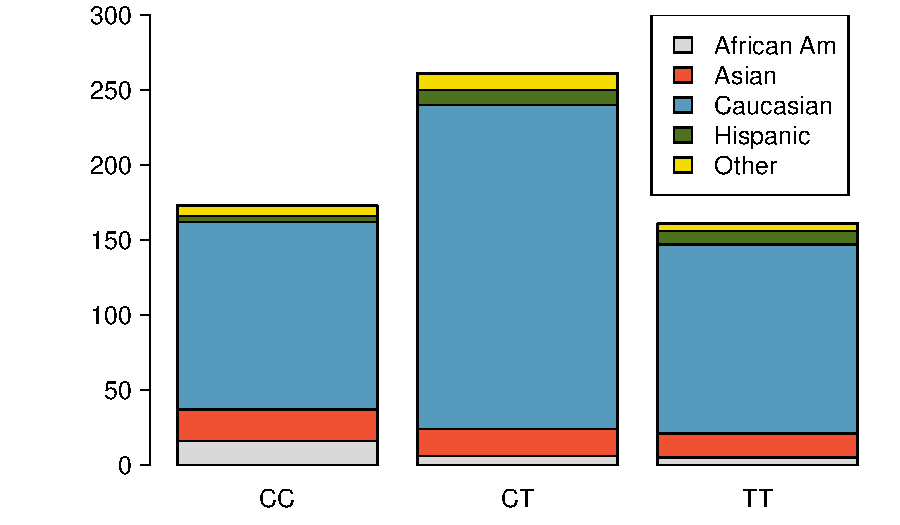
\includegraphics{figures/famussSegBarA.pdf}
								\caption{alt text}
							\end{figure}
							
							\emph{OI Biostat} Figure 1.35a, segmented bar plot
							
						\end{frame}
						
						\begin{frame}{Two categorical variables \dots}
							\protect\hypertarget{two-categorical-variables-3}{}
							
							\begin{figure}
								\centering
								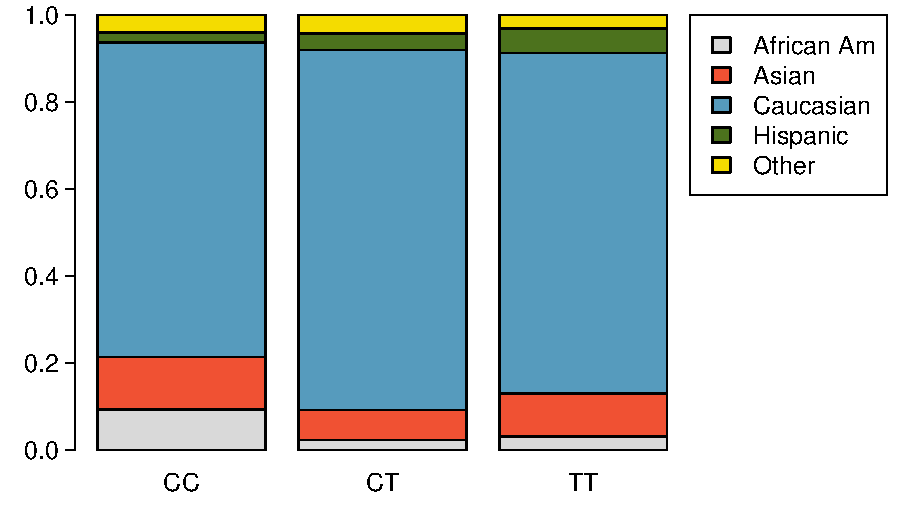
\includegraphics{figures/famussSegBarStaA.pdf}
								\caption{standardized segmented barplots}
							\end{figure}
							
							\emph{OI Biostat} Figure 1.35b, standardized segmented bar plot
							
						\end{frame}
						
						\begin{frame}{Two categorical variables \dots}
							\protect\hypertarget{two-categorical-variables-4}{}
							
							\emph{Relative risk} (RR) is one way of summarizing data presented in a
							two-way table of study outcome by participant group.
							
							More in Lab 1 \dots
							
						\end{frame}
						
						\begin{frame}{A numerical variable and a categorical variable}
							\protect\hypertarget{a-numerical-variable-and-a-categorical-variable}{}
							
							\emph{FAMuSS} was designed to study the relationship between genotype at
							the location \emph{r577x} in the gene \emph{ACTN3} and muscle strength.
							
							Muscle strength was assessed by the percent change in non-dominant arm
							strength after resistance training (\texttt{ndrm.ch}).
							
							What visualization would be a good choice to make this comparison?
							
						\end{frame}
						
						\begin{frame}[fragile]{A numerical variable and a categorical variable
								\dots}
							\protect\hypertarget{a-numerical-variable-and-a-categorical-variable-1}{}
							
							\scriptsize
							
							\scriptsize
							
\begin{knitrout}\scriptsize
\definecolor{shadecolor}{rgb}{0.969, 0.969, 0.969}\color{fgcolor}\begin{kframe}
\begin{alltt}
\hlkwd{boxplot}\hlstd{(famuss}\hlopt{$}\hlstd{ndrm.ch} \hlopt{~} \hlstd{famuss}\hlopt{$}\hlstd{actn3.r577x)}
\end{alltt}
\end{kframe}

{\centering 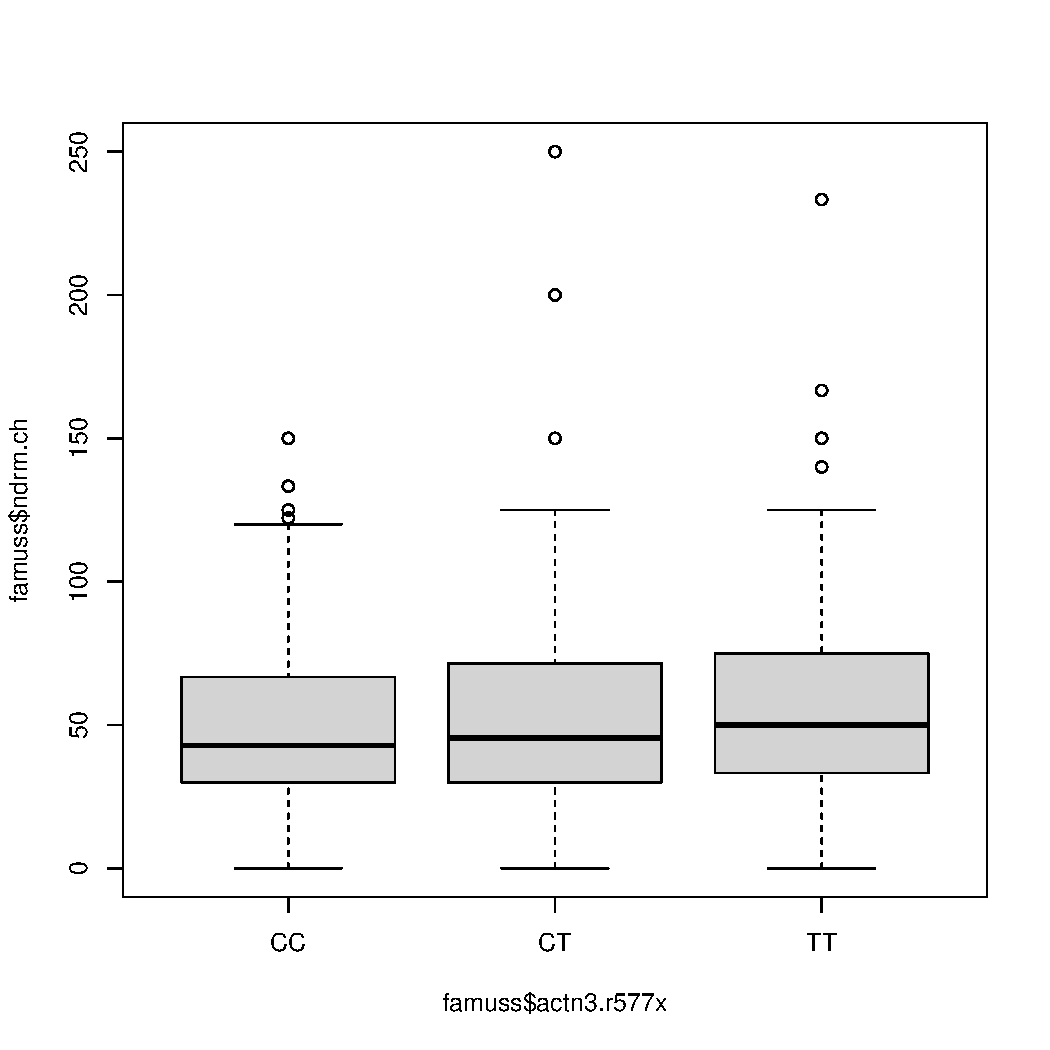
\includegraphics[width=\maxwidth]{figure/box-1-1} 

}


\end{knitrout}
							
							
							\normalsize
							
						\end{frame}
						
						\hypertarget{case-study-molecular-cancer-classification}{%
							\section{Case study: molecular cancer
								classification}\label{case-study-molecular-cancer-classification}}
						
						\begin{frame}{The potential value of genomic data in cancer}
							\protect\hypertarget{the-potential-value-of-genomic-data-in-cancer}{}
							
							The majority of cancers are diagnosed by an expert pathologist examining
							slides of malignant cells.
							
							Can that be done more accurately by characterizing the genetic makeup of
							the malignancy?
							
							\begin{itemize}
								\tightlist
								\item
								This is perhaps the major potential of genomic characterizations of
								tumors.
							\end{itemize}
							
							There are many forms of childhood leukemia.
							
							\begin{itemize}
								\item
								Acute myeloblastic leukemia (AML) and acute lymphoblastic leukemia
								(ALL) are the most common.
								\item
								AML is a cancer of the bone marrow, where white blood cells
								(lymphocytes) are produced.
								\item
								ALL is a cancer of the lymphocytes and is designated as B-cell (ALLB)
								or T-cell (ALLT).
							\end{itemize}
							
						\end{frame}
						
						\begin{frame}{Prognosis of the two cancers}
							\protect\hypertarget{prognosis-of-the-two-cancers}{}
							
							The probability that a child diagnosed with ALL is survives at least 5
							years after the diagnosis is approximately 90\%.
							
							Approximately 65\% of children diagnosed with AML survive at least 5
							years.
							
							The diagnosis of leukemia type determines the therapy that will be given
							to the child, and the successful treatments for ALL and AML are
							different.
							
							In 1999, Todd Golub from the Dana-Farber and the Broad Institute
							examined the possibility of classifying leukemia through using a genetic
							analysis of a blood sample.
							
						\end{frame}
						
						\begin{frame}{Analyzing the Golub data}
							\protect\hypertarget{analyzing-the-golub-data}{}
							
							We can re-analyze the Golub data using tools from graphical and
							numerical summaries.
							
							Our analysis will not be identical to the Golub analysis, but will be
							similar in spirit.
							
							The tools are straighforward\ldots   
							
							\begin{itemize}
								\item
								Thinking through the problem and assembling the tools is the hard
								part.
								\item
								The process is more important than the final recipe.
							\end{itemize}
							
						\end{frame}
						
						\begin{frame}{Gene expression (details in \emph{OI Biostat})}
							\protect\hypertarget{gene-expression-details-in-oi-biostat}{}
							
							\small
							
							\begin{itemize}
								\item
								The genetic code stored in DNA contains the information for producing
								the proteins that determine an organism's phenotype.
								\item
								Genes that are transcriptionally active (i.e.~turned ``on'') are
								transcribed into messenger RNA (mRNA) that gets translated into
								proteins.
								\item
								Genes can be switched on or off, and expressed at varying levels.
								Variations in gene expression produce the range of physical,
								biochemical, and developmental differences in cells and tissues.
								\item
								Quantifying the amount of RNA produced in a cell allows for a measure
								of gene expression.
								\item
								The transcriptome, or expression profile, is the complete set of RNA
								transcripts produced by the genome in a cell or set of cells.
							\end{itemize}
							
						\end{frame}
						
						\begin{frame}{Microarrays (details in \emph{OI Biostat})}
							\protect\hypertarget{microarrays-details-in-oi-biostat}{}
							
							\small
							
							\begin{itemize}
								\item
								Microarray technology is based on hybridization between two DNA
								strands, in which complementary nucleotide sequences specifically pair
								together.
								\item
								The mRNA from a sample is converted into complementary-DNA (cDNA),
								labeled with a fluorescent dye, and added to the microarray.
								\item
								When cDNA from the sample encounters complementary DNA probes, the two
								strands will hybridize, allowing the cDNA to adhere to specific spots
								on the slide.
								\item
								When the chip is illuminated and scanned, the intensity of
								fluorescence detected at each spot corresponds to the amount of bound
								cDNA.
								\item
								DNA microarrays do not directly quantify gene expression levels or
								quantity of mRNA present in a sample.
								\item
								The fluorescence intensity data only provide a relative measure of
								gene expression, showing which genes on the chip seem to be more or
								less active in relation to each other.
							\end{itemize}
							
						\end{frame}
						
						\begin{frame}{Microarrays}
							\protect\hypertarget{microarrays}{}
							
							\begin{figure}
								\centering
								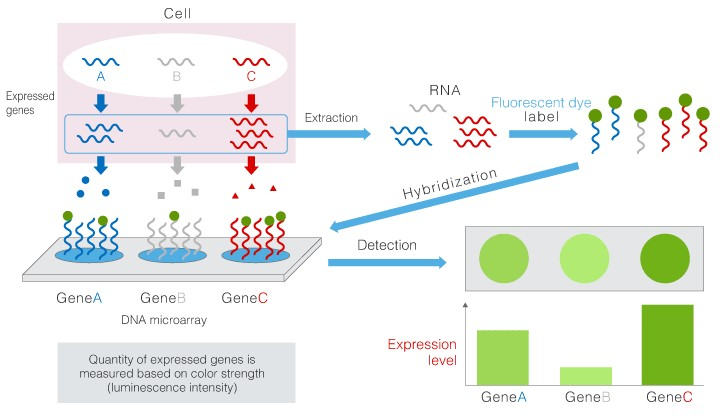
\includegraphics{figures/microarray_schematic.jpg}
								\caption{fluorescence detection}
							\end{figure}
							
						\end{frame}
						
						\begin{frame}{The Golub clinical data}
							\protect\hypertarget{the-golub-clinical-data}{}
							
							Demographic variables described in \emph{OI Biostat} Table 1.54:
							
							\scriptsize
							
							\begin{longtable}[]{@{}ll@{}}
								\toprule
								\begin{minipage}[b]{0.12\columnwidth}\raggedright
									Variable\strut
								\end{minipage} & \begin{minipage}[b]{0.82\columnwidth}\raggedright
									Description\strut
								\end{minipage}\tabularnewline
								\midrule
								\endhead
								\begin{minipage}[t]{0.12\columnwidth}\raggedright
									Samples\strut
								\end{minipage} & \begin{minipage}[t]{0.82\columnwidth}\raggedright
									Sample or chip number. The material from each patient was examined on a
									separate chip and experimental run.\strut
								\end{minipage}\tabularnewline
								\begin{minipage}[t]{0.12\columnwidth}\raggedright
									BM.PB\strut
								\end{minipage} & \begin{minipage}[t]{0.82\columnwidth}\raggedright
									Type of patient material. BM denotes bone marrow; PB denotes a
									peripheral blood sample.\strut
								\end{minipage}\tabularnewline
								\begin{minipage}[t]{0.12\columnwidth}\raggedright
									Gender\strut
								\end{minipage} & \begin{minipage}[t]{0.82\columnwidth}\raggedright
									F for female, M for male.\strut
								\end{minipage}\tabularnewline
								\begin{minipage}[t]{0.12\columnwidth}\raggedright
									Source\strut
								\end{minipage} & \begin{minipage}[t]{0.82\columnwidth}\raggedright
									Hospital where the patient was treated.\strut
								\end{minipage}\tabularnewline
								\begin{minipage}[t]{0.12\columnwidth}\raggedright
									tissue.mf\strut
								\end{minipage} & \begin{minipage}[t]{0.82\columnwidth}\raggedright
									A variable showing the combination of type of patient material and sex
									of the patient. BM:f denotes bone marrow from a female patient,
									etc.\strut
								\end{minipage}\tabularnewline
								\begin{minipage}[t]{0.12\columnwidth}\raggedright
									cancer\strut
								\end{minipage} & \begin{minipage}[t]{0.82\columnwidth}\raggedright
									The type of leukemia; aml is acute myeloblastic leukemia, allB is acute
									lymphoblastic leukemia which started in B-cells (cells that mature into
									plasma cells) origin, and allT is acute lymphoblastic leukemia with
									T-cell origin (T-cells are a type of white blood cell).\strut
								\end{minipage}\tabularnewline
								\bottomrule
							\end{longtable}
							
						\end{frame}
						
						\begin{frame}{The Golub expression data}
							\protect\hypertarget{the-golub-expression-data}{}
							
							The expression data is contained in the last 7,129 columns.
							
							Each column is a variable with a name corresponding to the name of the
							probe on the microarray.
							
							The expression levels record fluorescence intensity for each gene.
							
							\begin{itemize}
								\item
								The intensity levels have no inherent biological meaning.
								\item
								Data have been normalized to adjust for variability between the
								separate arrays used for each patient.
							\end{itemize}
							
						\end{frame}
						
						\begin{frame}{Selected variables and columns from Golub data}
							\protect\hypertarget{selected-variables-and-columns-from-golub-data}{}
							
							\captionsetup[table]{labelformat=empty}
							\scriptsize
							
							\scriptsize
							
							\begin{longtable}[]{@{}rllrrr@{}}
								\caption{\emph{OI Biostat} Table 1.40}\tabularnewline
								\toprule
								Samples & Gender & cancer & AFFX-BioB-5\_at & AFFX-BioB-M\_at &
								AFFX-BioB-3\_at\tabularnewline
								\midrule
								\endfirsthead
								\toprule
								Samples & Gender & cancer & AFFX-BioB-5\_at & AFFX-BioB-M\_at &
								AFFX-BioB-3\_at\tabularnewline
								\midrule
								\endhead
								39 & F & allB & -1363.28 & -1058.59 & -541.47\tabularnewline
								40 & F & allB & -796.29 & -1167.10 & 7.54\tabularnewline
								42 & F & allB & -679.14 & -1069.83 & -690.30\tabularnewline
								47 & M & allB & -1164.40 & -1109.94 & -990.13\tabularnewline
								48 & F & allB & -1299.65 & -1402.00 & -1077.54\tabularnewline
								\bottomrule
							\end{longtable}
							
							\normalsize
							
						\end{frame}
						
						\begin{frame}{Analyzing the Golub leukemia data}
							\protect\hypertarget{analyzing-the-golub-leukemia-data}{}
							
							We will do an analysis in class using some of the simple but
							surprisingly powerful ideas behind numerical and graphical summaries.
							
							The goal of the Golub study was to develop a procedure for
							distinguishing between AML and ALL based only on the gene expression
							levels of a patient. There are two major issues to be addressed:
							
							\begin{enumerate}
								\item
								Which genes are the most informative for making a prediction?
								\item
								What is a workable strategy for predicting leukemia type from
								expression data for a specific set of genes?
							\end{enumerate}
							
						\end{frame}
						
						\begin{frame}[fragile]{Starting small\ldots{}}
							\protect\hypertarget{starting-small}{}
							
							\footnotesize
							
							\scriptsize
							
							\begin{verbatim}
							##    cancer        A         B        C        D
							## 69   allB 39307.96 35232.401 41170.76 35792.79
							## 67   allT 32281.88 41432.024 59328.51 49608.14
							## 55   allB 47429.94 35568.928 56074.96 42857.78
							## 56   allB 25533.87 16983.749 28056.75 32693.92
							## 59   allB 35960.55 24191.746 27637.90 22240.75
							## 52    aml 46177.95  6189.465 12557.24 34485.41
							## 53    aml 43790.70 33661.825 38380.30 29758.25
							## 51    aml 53420.05 26109.245 31427.20 23809.70
							## 50    aml 41241.59 37589.773 47325.77 30099.36
							## 54    aml 41300.57 49198.412 66026.10 56248.62
							\end{verbatim}
							
							\normalsize
							
						\end{frame}
						
\end{document}






\begin{frame}[fragile]{What levels of immunity are found in patients who have recovered from  COVID-19?\footnote{\tiny{Data were (imperfectly) scraped from the Postscript file ``behind'' the pdf file by Dr. Hanley}} }

	
\begin{knitrout}\tiny
\definecolor{shadecolor}{rgb}{0.969, 0.969, 0.969}\color{fgcolor}\begin{kframe}
\begin{alltt}
\hlstd{path} \hlkwb{<-}
  \hlstr{"http://www.biostat.mcgill.ca/hanley/statbook/immunogenicityChAdOx1.nCoV-19vaccine.txt"}
\hlstd{ds} \hlkwb{<-} \hlkwd{read.table}\hlstd{(path)}
\hlkwd{head}\hlstd{(ds)}
\end{alltt}
\begin{verbatim}
##   RefIndexCategory IgGResponse.log10.ElisaUnits
## 1     Convalescent                         2.56
## 2     Convalescent                         2.74
## 3     Convalescent                         2.79
## 4     Convalescent                         3.32
## 5     Convalescent                         3.15
## 6     Convalescent                         2.35
\end{verbatim}
\begin{alltt}
\hlkwd{str}\hlstd{(ds)}
\end{alltt}
\begin{verbatim}
## 'data.frame':	307 obs. of  2 variables:
##  $ RefIndexCategory            : chr  "Convalescent" "Convalescent" "Convalescent" "Convalescent" ...
##  $ IgGResponse.log10.ElisaUnits: num  2.56 2.74 2.79 3.32 3.15 2.35 2.72 2.95 2.42 2.64 ...
\end{verbatim}
\begin{alltt}
\hlkwd{levels}\hlstd{(ds}\hlopt{$}\hlstd{RefIndexCategory)}
\end{alltt}
\begin{verbatim}
## NULL
\end{verbatim}
\end{kframe}
\end{knitrout}

\end{frame}



\begin{frame}[fragile]{What levels of immunity are found in patients who have recovered from  COVID-19?}


\begin{knitrout}\tiny
\definecolor{shadecolor}{rgb}{0.969, 0.969, 0.969}\color{fgcolor}\begin{kframe}
\begin{alltt}
\hlstd{natural} \hlkwb{<-} \hlstd{ds[ds}\hlopt{$}\hlstd{RefIndexCategory}\hlopt{==}\hlstr{"Convalescent"}\hlstd{,]}
\hlkwd{hist}\hlstd{(natural}\hlopt{$}\hlstd{IgGResponse.log10.ElisaUnits,}
     \hlkwc{breaks} \hlstd{=} \hlnum{20}\hlstd{,} \hlkwc{col} \hlstd{=} \hlstr{"lightblue"}\hlstd{)}
\end{alltt}
\end{kframe}

{\centering 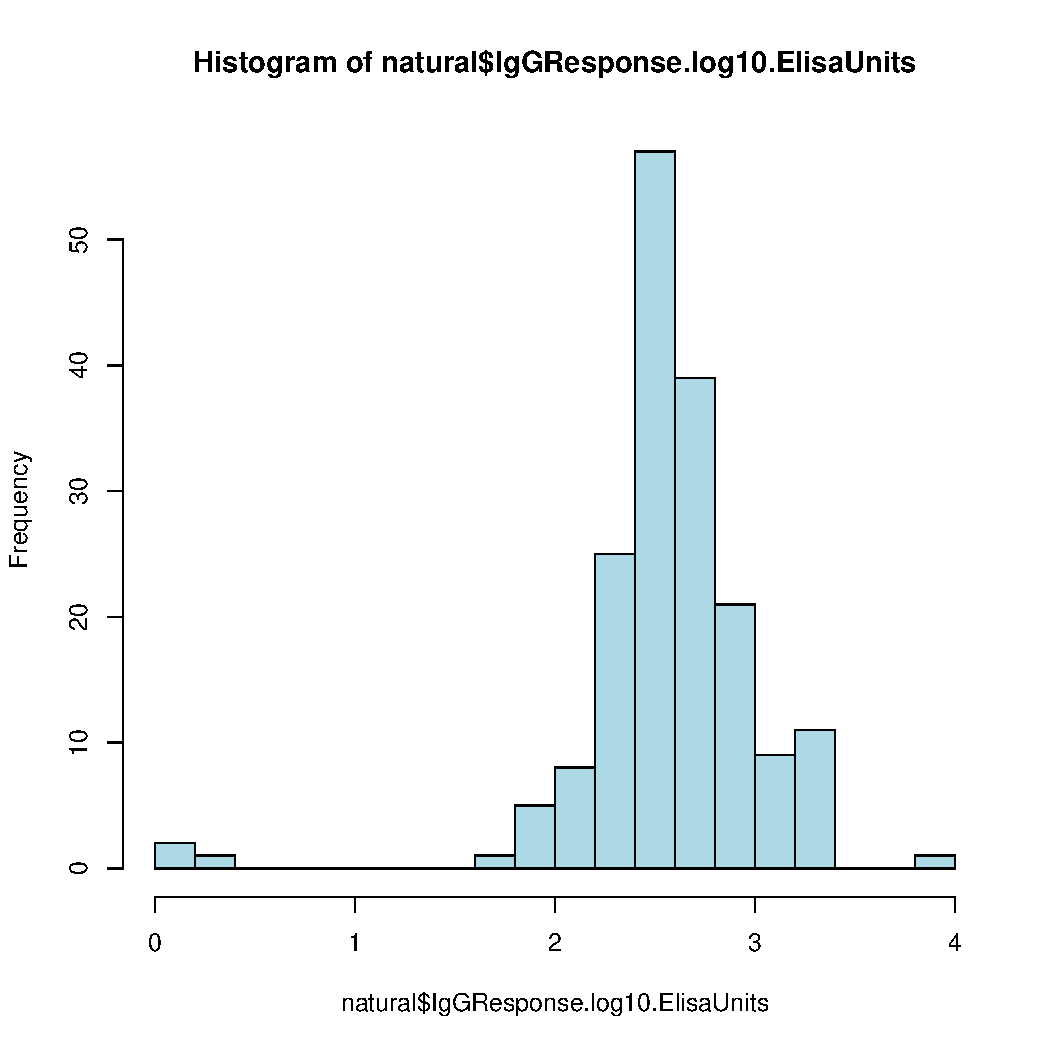
\includegraphics[width=0.6\linewidth]{figure/unnamed-chunk-3-1} 

}


\end{knitrout}

\end{frame}


\begin{frame}[fragile]{Three different methods of calculating the mean}

\begin{figure}
\begin{minipage}[h]{0.40\linewidth}
\begin{knitrout}\tiny
\definecolor{shadecolor}{rgb}{0.969, 0.969, 0.969}\color{fgcolor}\begin{kframe}
\begin{alltt}
\hlkwd{summary}\hlstd{(natural}\hlopt{$}\hlstd{IgGResponse.log10.ElisaUnits)}
\end{alltt}
\begin{verbatim}
##    Min. 1st Qu.  Median    Mean 3rd Qu.    Max. 
##   0.000   2.417   2.570   2.577   2.780   3.860
\end{verbatim}
\begin{alltt}
\hlkwd{boxplot}\hlstd{(natural}\hlopt{$}\hlstd{IgGResponse.log10.ElisaUnits,}
        \hlkwc{col} \hlstd{=} \hlstr{"lightblue"}\hlstd{,}
        \hlkwc{ylab} \hlstd{=} \hlstr{"Immunoglobulin G (IgG) response"}\hlstd{)}
\hlkwd{grid}\hlstd{(}\hlkwc{lty} \hlstd{=} \hlstr{"dashed"}\hlstd{)}
\end{alltt}
\end{kframe}

{\centering 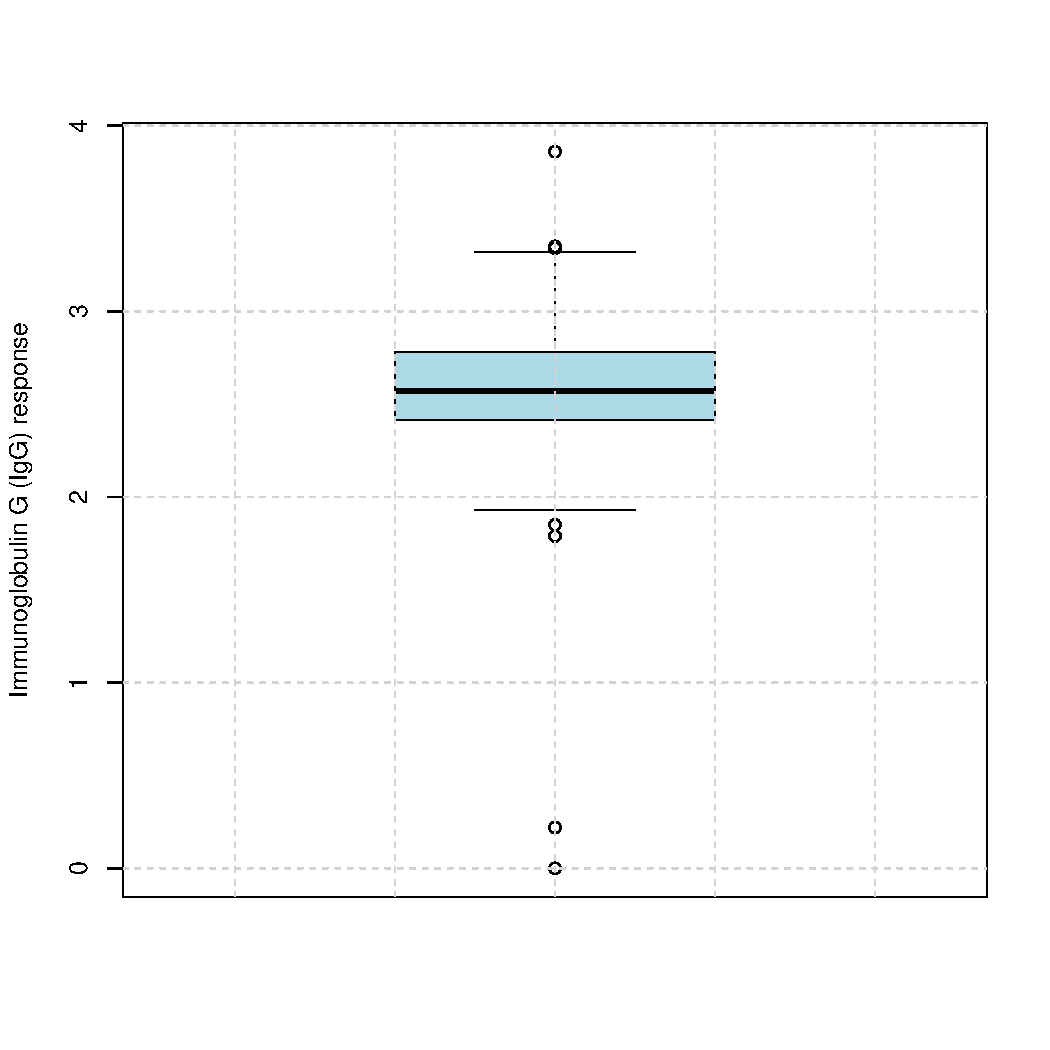
\includegraphics[width=0.99\linewidth]{figure/unnamed-chunk-4-1} 

}


\end{knitrout}

\end{minipage}
\hspace{0.4cm}
\begin{minipage}[h]{0.50\linewidth}
\begin{knitrout}\tiny
\definecolor{shadecolor}{rgb}{0.969, 0.969, 0.969}\color{fgcolor}\begin{kframe}
\begin{alltt}
\hlkwd{t.test}\hlstd{(natural}\hlopt{$}\hlstd{IgGResponse.log10.ElisaUnits)}
\end{alltt}
\begin{verbatim}
## One Sample t-test with natural$IgGResponse.log10.ElisaUnits 
## t = 75.0898, df = 179, p-value < 2.2e-16
## alternative hypothesis: true mean is not equal to 0 
## 95 percent confidence interval:
##  2.509603 2.645064 
## sample estimates:
## mean of x 
##  2.577333
\end{verbatim}
\begin{alltt}
\hlstd{fit1} \hlkwb{<-} \hlkwd{glm}\hlstd{(IgGResponse.log10.ElisaUnits} \hlopt{~} \hlnum{1}\hlstd{,} \hlkwc{data} \hlstd{= natural)}
\hlkwd{summary}\hlstd{(fit1)}
\end{alltt}
\begin{verbatim}
## 
## Coefficients:
##             Estimate Std. Error t value Pr(>|t|)    
## (Intercept)  2.57733    0.03432   75.09   <2e-16 ***
## ---
## Signif. codes:  0 '***' 0.001 '**' 0.01 '*' 0.05 '.' 0.1 ' ' 1
## 
## (Dispersion parameter for gaussian family taken to be 0.2120565)
## 
##     Null deviance: 37.958  on 179  degrees of freedom
## Residual deviance: 37.958  on 179  degrees of freedom
## AIC: 234.65
## 
## Number of Fisher Scoring iterations: 2
\end{verbatim}
\begin{alltt}
\hlkwd{confint}\hlstd{(fit1)}
\end{alltt}
\begin{verbatim}
##    2.5 %   97.5 % 
## 2.510061 2.644606
\end{verbatim}
\end{kframe}
\end{knitrout}
\end{minipage}
\end{figure}


\end{frame}



\begin{frame}[fragile]{Naturally vs. vaccine-induced response levels}
	
	
\begin{knitrout}\tiny
\definecolor{shadecolor}{rgb}{0.969, 0.969, 0.969}\color{fgcolor}\begin{kframe}
\begin{alltt}
\hlstd{p1} \hlkwb{<-} \hlkwd{ggplot}\hlstd{(}\hlkwc{data} \hlstd{= ds,} \hlkwc{mapping} \hlstd{=} \hlkwd{aes}\hlstd{(}\hlkwc{x} \hlstd{= RefIndexCategory,} \hlkwc{y} \hlstd{= IgGResponse.log10.ElisaUnits,}
    \hlkwc{fill} \hlstd{= RefIndexCategory))} \hlopt{+} \hlkwd{geom_jitter}\hlstd{(}\hlkwc{alpha} \hlstd{=} \hlnum{0.3}\hlstd{)} \hlopt{+} \hlkwd{theme_minimal}\hlstd{()} \hlopt{+} \hlkwd{theme}\hlstd{(}\hlkwc{legend.position} \hlstd{=} \hlstr{"none"}\hlstd{)}
\hlstd{p1} \hlopt{+} \hlkwd{geom_violin}\hlstd{()}
\hlstd{p1} \hlopt{+} \hlkwd{geom_boxplot}\hlstd{()}
\end{alltt}
\end{kframe}\begin{figure}

{\centering \subfloat[Violin plot\label{fig:unnamed-chunk-6-1}]{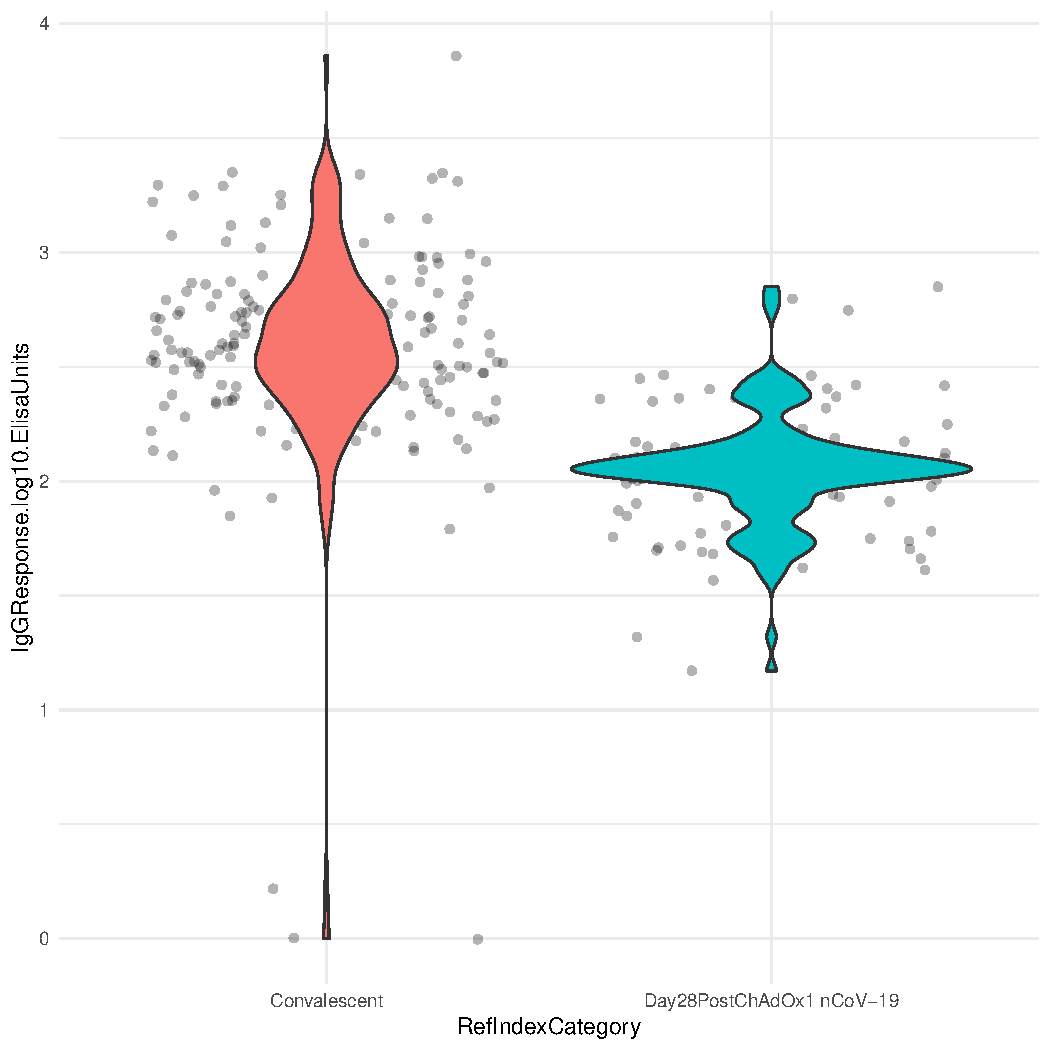
\includegraphics[width=0.5\linewidth]{figure/unnamed-chunk-6-1} }
\subfloat[Boxplot\label{fig:unnamed-chunk-6-2}]{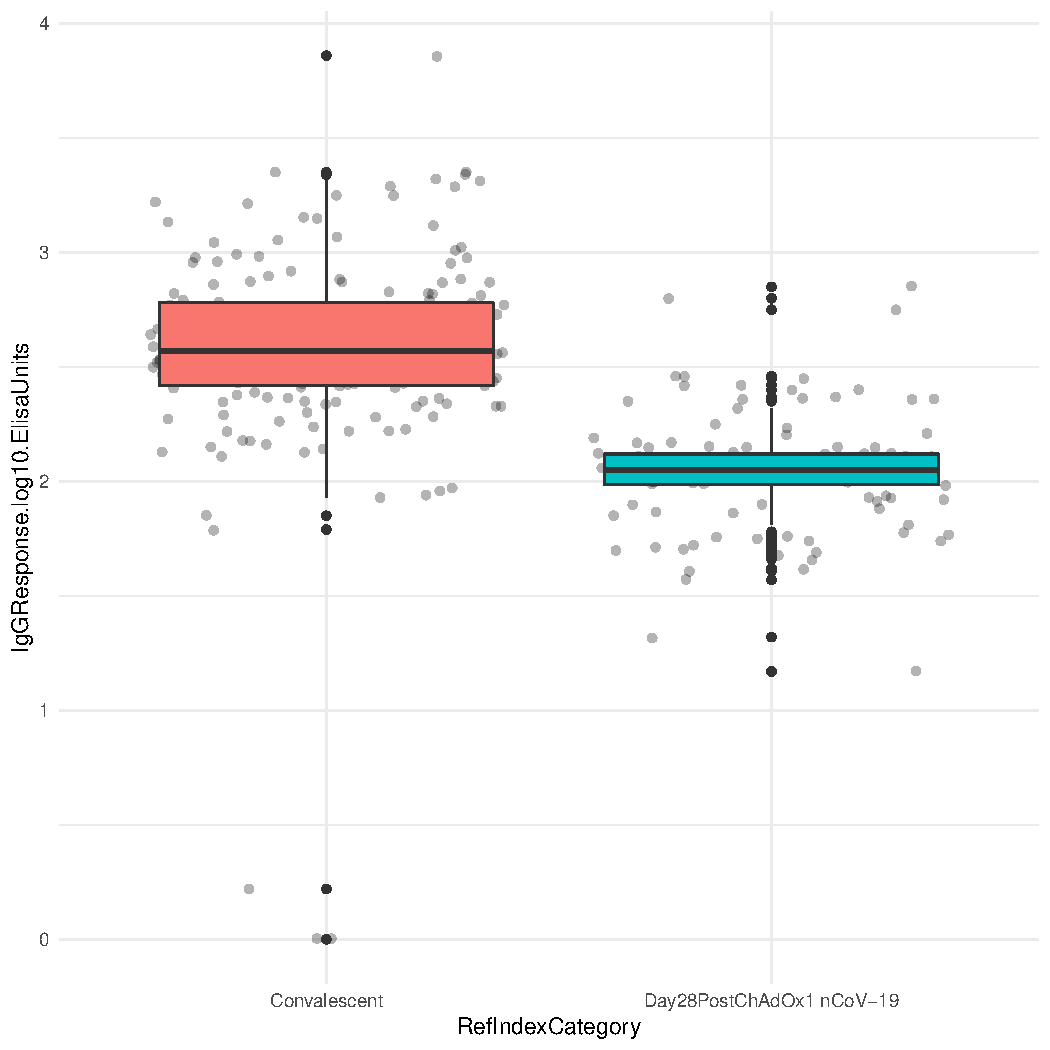
\includegraphics[width=0.5\linewidth]{figure/unnamed-chunk-6-2} }

}

\end{figure}

\end{knitrout}
	
\end{frame}



\begin{frame}[fragile]{Comparing means using classic methods}

\textbf{1. Numerical summary} \\

\begin{knitrout}\tiny
\definecolor{shadecolor}{rgb}{0.969, 0.969, 0.969}\color{fgcolor}\begin{kframe}
\begin{alltt}
\hlkwd{by}\hlstd{(ds}\hlopt{$}\hlstd{IgGResponse.log10.ElisaUnits,ds}\hlopt{$}\hlstd{RefIndexCategory,summary)}
\end{alltt}
\begin{verbatim}
## ds$RefIndexCategory: Convalescent
##    Min. 1st Qu.  Median    Mean 3rd Qu.    Max. 
##   0.000   2.417   2.570   2.577   2.780   3.860 
## ------------------------------------------------------------ 
## ds$RefIndexCategory: Day28PostChAdOx1 nCoV-19
##    Min. 1st Qu.  Median    Mean 3rd Qu.    Max. 
##   1.170   1.985   2.050   2.047   2.120   2.850
\end{verbatim}
\end{kframe}
\end{knitrout}
\pause

\vspace*{0.3in}

\textbf{2. Another ``dot'' test} \\

\begin{knitrout}\tiny
\definecolor{shadecolor}{rgb}{0.969, 0.969, 0.969}\color{fgcolor}\begin{kframe}
\begin{alltt}
\hlkwd{t.test}\hlstd{(IgGResponse.log10.ElisaUnits} \hlopt{~} \hlstd{RefIndexCategory,} \hlkwc{data} \hlstd{= ds)}
\end{alltt}


{\ttfamily\noindent\bfseries\color{errorcolor}{\#\# Error in mosaic\_formula\_q(formula, groups = groups, max.slots = 2, envir = if (is.environment(data)) data else environment(formula)): Invalid formula specification. \ Too many slots (3>2).}}\end{kframe}
\end{knitrout}

\end{frame}



\begin{frame}[fragile]{Comparing means using regression}
	
\textbf{3. Regression} \\
	
\begin{knitrout}\tiny
\definecolor{shadecolor}{rgb}{0.969, 0.969, 0.969}\color{fgcolor}\begin{kframe}
\begin{alltt}
\hlstd{fit2} \hlkwb{<-} \hlkwd{glm}\hlstd{(IgGResponse.log10.ElisaUnits} \hlopt{~} \hlstd{RefIndexCategory,} \hlkwc{data} \hlstd{= ds)}
\hlkwd{print}\hlstd{(}\hlkwd{summary}\hlstd{(fit2),} \hlkwc{signif.star} \hlstd{=} \hlnum{FALSE}\hlstd{)}
\end{alltt}
\begin{verbatim}
## 
## Coefficients:
##                                          Estimate Std. Error t value Pr(>|t|)
## (Intercept)                               2.57733    0.02874   89.67   <2e-16
## RefIndexCategoryDay28PostChAdOx1 nCoV-19 -0.53080    0.04469  -11.88   <2e-16
## 
## (Dispersion parameter for gaussian family taken to be 0.1487187)
## 
##     Null deviance: 66.339  on 306  degrees of freedom
## Residual deviance: 45.359  on 305  degrees of freedom
## AIC: 290.17
## 
## Number of Fisher Scoring iterations: 2
\end{verbatim}
\begin{alltt}
\hlkwd{confint}\hlstd{(fit2)}
\end{alltt}
\begin{verbatim}
##                                               2.5 %     97.5 %
## (Intercept)                               2.5209962  2.6336704
## RefIndexCategoryDay28PostChAdOx1 nCoV-19 -0.6183894 -0.4432064
\end{verbatim}
\end{kframe}
\end{knitrout}

\end{frame}


\begin{frame}[fragile]{Fitted regression line}
	
\begin{knitrout}\tiny
\definecolor{shadecolor}{rgb}{0.969, 0.969, 0.969}\color{fgcolor}\begin{kframe}
\begin{alltt}
\hlkwd{plot}\hlstd{(ds}\hlopt{$}\hlstd{RefIndexCategory, ds}\hlopt{$}\hlstd{IgGResponse.log10.ElisaUnits,} \hlkwc{pch}\hlstd{=}\hlnum{19}\hlstd{,} \hlkwc{cex}\hlstd{=}\hlnum{0.5}\hlstd{)}
\end{alltt}


{\ttfamily\noindent\bfseries\color{errorcolor}{\#\# Error in plot.window(...): need finite 'xlim' values}}\end{kframe}\begin{figure}

{\centering 
\includegraphics[width=0.5\linewidth]{figure/unnamed-chunk-10-1} 

}

\caption[The red line is the fitted regression from the previous slide]{The red line is the fitted regression from the previous slide.}\label{fig:unnamed-chunk-10}
\end{figure}

\begin{kframe}\begin{alltt}
\hlkwd{abline}\hlstd{(}\hlkwc{h} \hlstd{=} \hlkwd{seq}\hlstd{(}\hlnum{0}\hlstd{,}\hlnum{4}\hlstd{,}\hlnum{0.5}\hlstd{),}\hlkwc{col} \hlstd{=} \hlstr{"lightblue"}\hlstd{)}
\hlkwd{lines}\hlstd{(ds}\hlopt{$}\hlstd{RefIndexCategory, fit2}\hlopt{$}\hlstd{fitted.values,} \hlkwc{col} \hlstd{=} \hlstr{"red"}\hlstd{,} \hlkwc{lwd} \hlstd{=} \hlnum{3}\hlstd{)}
\end{alltt}
\end{kframe}
\end{knitrout}
	
\end{frame}




\section{Case study 2: Comparison of Estimated Rates of Coronavirus Disease 2019 (COVID-19) in Border Counties in Iowa Without a Stay-at-Home Order and Border Counties in Illinois With a Stay-at-Home Order}

\begin{frame}{Comparing Iowa and Illinois Cases\footnote{\tiny\url{https://jamanetwork.com/journals/jamanetworkopen/fullarticle/2766229}}}
	\centering
	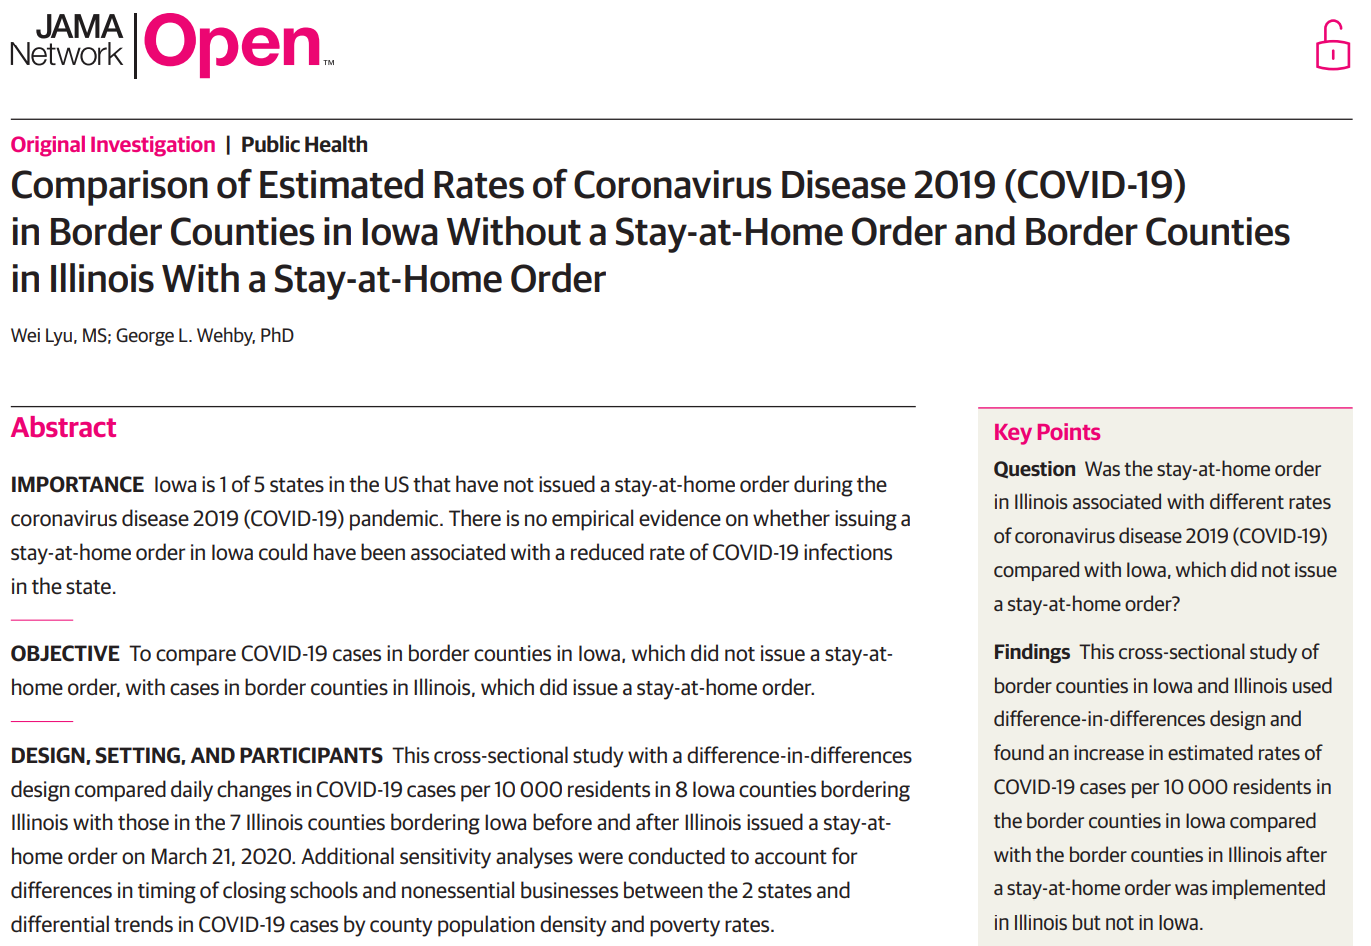
\includegraphics[scale=0.25]{002-masks.png}	
\end{frame}


\begin{frame}[fragile]{Are the difference in curves real? Or just random variation?}

\begin{itemize}
	\item This study compared COVID-19 cases in border counties in \textcolor{red}{Iowa, which did not issue a stay-at-home order}, with cases in border counties in \textcolor{blue}{Illinois, which did issue a stay-at-home order}.
\end{itemize}

\begin{knitrout}\tiny
\definecolor{shadecolor}{rgb}{0.969, 0.969, 0.969}\color{fgcolor}

{\centering 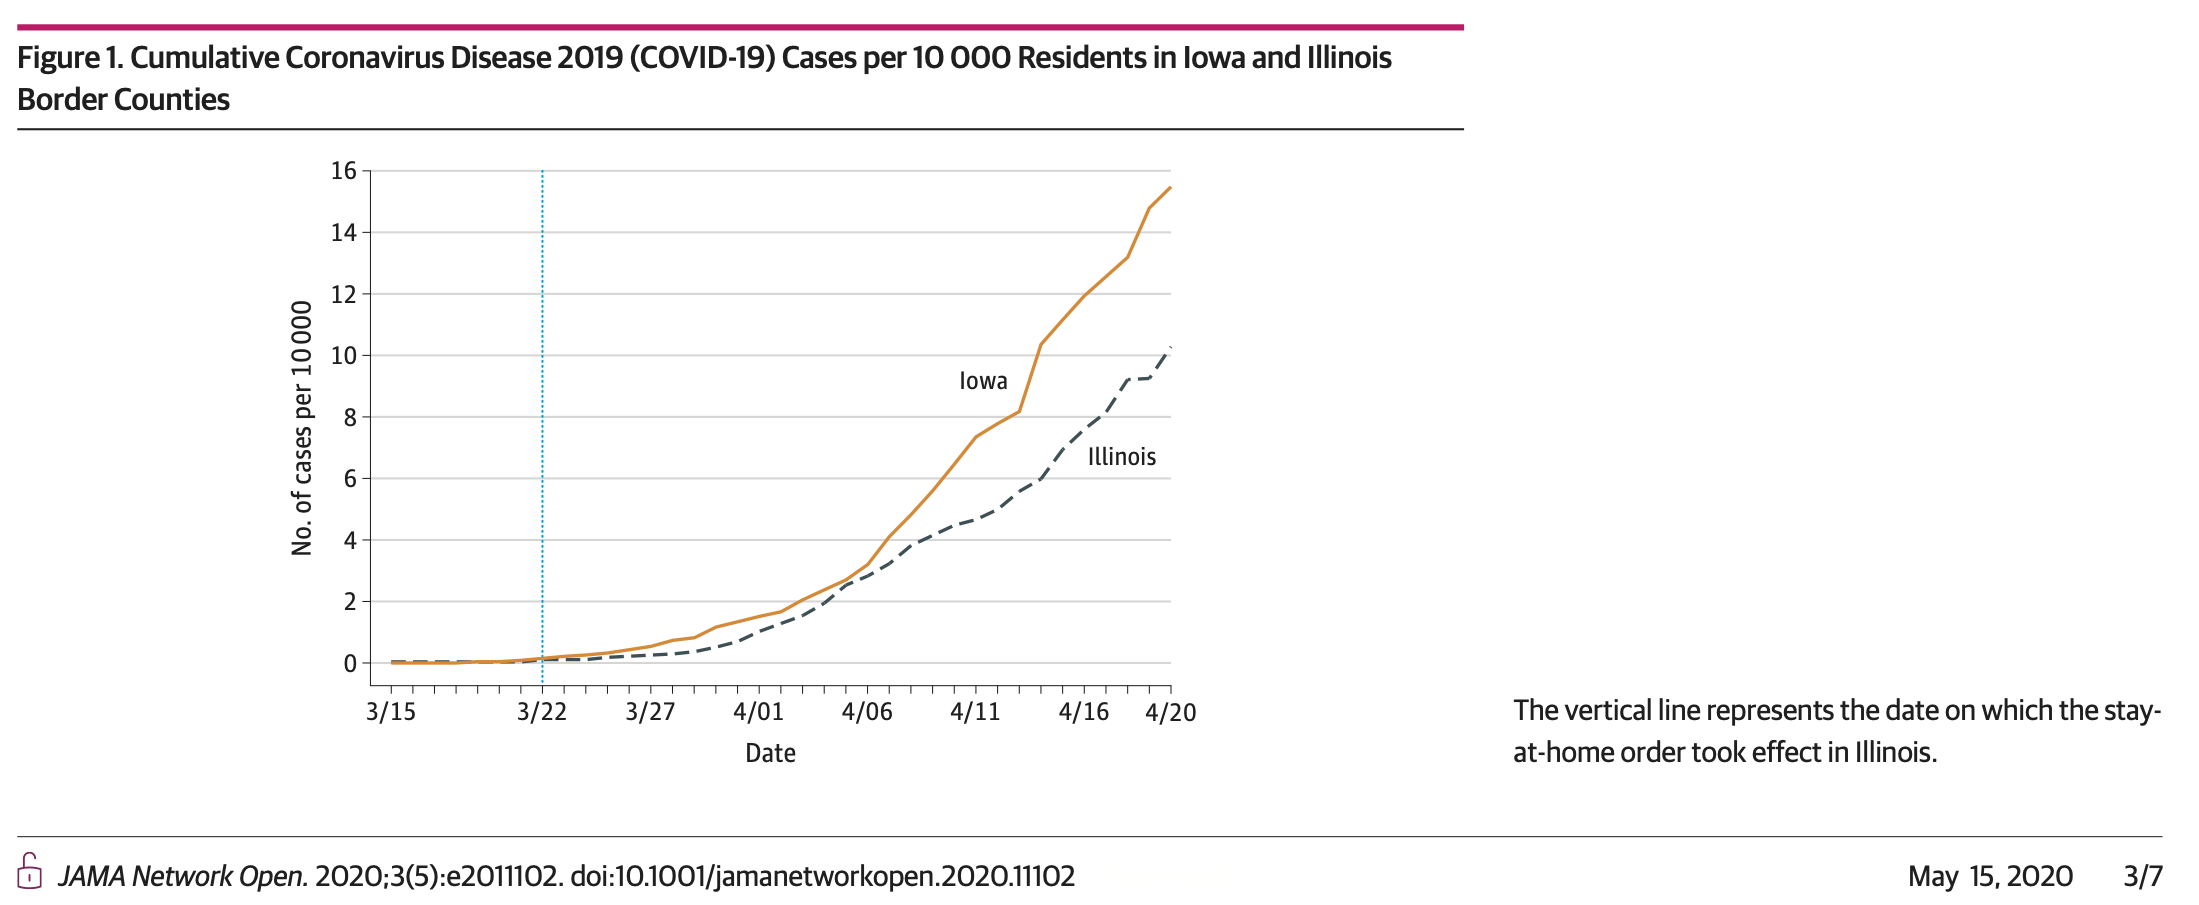
\includegraphics[width=1\linewidth]{downloadFigs4latex_003-exploring-data-1_slides/masks} 

}


\end{knitrout}

\end{frame}





\begin{frame}[fragile]{Freely available county level data from NYTimes\footnote{\tiny{\url{https://github.com/nytimes/covid-19-data}}}}
	
\begin{knitrout}\tiny
\definecolor{shadecolor}{rgb}{0.969, 0.969, 0.969}\color{fgcolor}\begin{kframe}
\begin{alltt}
\hlkwd{library}\hlstd{(covdata)} \hlcom{# remotes::install_github("kjhealy/covdata")}
\hlkwd{library}\hlstd{(dplyr);} \hlkwd{library}\hlstd{(tidyr);} \hlkwd{library}\hlstd{(ggplot2);} \hlkwd{library}\hlstd{(readr)}

\hlcom{# get population data from https://covid19.census.gov/datasets/}
\hlstd{pop_county} \hlkwb{<-} \hlkwd{read_csv}\hlstd{(}\hlstr{"https://opendata.arcgis.com/datasets/21843f238cbb46b08615fc53e19e0daf_1.csv"}\hlstd{)} \hlopt
              \hlstd{dplyr}\hlopt{::}\hlkwd{rename}\hlstd{(}\hlkwc{fips} \hlstd{= GEOID,} \hlkwc{population} \hlstd{= B01001_001E,} \hlkwc{state} \hlstd{= State)} \hlopt
              \hlstd{dplyr}\hlopt{::}\hlkwd{select}\hlstd{(state, fips, population)}

\hlstd{county_level} \hlkwb{<-} \hlstd{nytcovcounty} \hlopt
                \hlstd{dplyr}\hlopt{::}\hlkwd{left_join}\hlstd{(pop_county,} \hlkwc{by} \hlstd{=} \hlkwd{c}\hlstd{(}\hlstr{"state"}\hlstd{,}\hlstr{"fips"}\hlstd{))} \hlopt
                \hlstd{dplyr}\hlopt{::}\hlkwd{mutate}\hlstd{(}\hlkwc{cases.per.10k} \hlstd{= cases}\hlopt{/}\hlstd{population} \hlopt{*} \hlnum{1e4}\hlstd{)} \hlopt
                \hlstd{dplyr}\hlopt{::}\hlkwd{filter}\hlstd{(state} \hlopt \hlkwd{c}\hlstd{(}\hlstr{"Iowa"}\hlstd{,}\hlstr{"Illinois"}\hlstd{))} \hlopt
                \hlstd{dplyr}\hlopt{::}\hlkwd{group_by}\hlstd{(county)}

\hlstd{pop_state} \hlkwb{<-} \hlstd{pop_county} \hlopt
             \hlstd{dplyr}\hlopt{::}\hlkwd{group_by}\hlstd{(state)} \hlopt
             \hlstd{dplyr}\hlopt{::}\hlkwd{summarise}\hlstd{(}\hlkwc{population} \hlstd{=} \hlkwd{sum}\hlstd{(population,} \hlkwc{na.rm} \hlstd{=} \hlnum{TRUE}\hlstd{))}

\hlstd{state_level} \hlkwb{<-} \hlstd{county_level} \hlopt
               \hlstd{dplyr}\hlopt{::}\hlkwd{group_by}\hlstd{(state, date)} \hlopt
               \hlstd{dplyr}\hlopt{::}\hlkwd{filter}\hlstd{(date} \hlopt{>=} \hlstr{"2020-03-15"}\hlstd{)} \hlopt
               \hlstd{dplyr}\hlopt{::}\hlkwd{summarise}\hlstd{(}\hlkwc{cases} \hlstd{=} \hlkwd{sum}\hlstd{(cases))} \hlopt
               \hlstd{dplyr}\hlopt{::}\hlkwd{left_join}\hlstd{(pop_state,} \hlkwc{by} \hlstd{=} \hlstr{"state"}\hlstd{)} \hlopt
               \hlstd{dplyr}\hlopt{::}\hlkwd{mutate}\hlstd{(}\hlkwc{cases.per.10k} \hlstd{= cases} \hlopt{/} \hlstd{population} \hlopt{*} \hlnum{1e4}\hlstd{,} \hlkwc{state} \hlstd{=} \hlkwd{factor}\hlstd{(state),}
                             \hlkwc{time} \hlstd{=} \hlkwd{as.numeric}\hlstd{(date} \hlopt{-} \hlkwd{min}\hlstd{(date))} \hlopt{+} \hlnum{1}\hlstd{)}
\hlkwd{head}\hlstd{(state_level)}
\end{alltt}
\begin{verbatim}
## # A tibble: 6 x 6
## # Groups:   state [1]
##   state    date       cases population cases.per.10k  time
##   <fct>    <date>     <dbl>      <dbl>         <dbl> <dbl>
## 1 Illinois 2020-03-15    94   12821497        0.0733     1
## 2 Illinois 2020-03-16   104   12821497        0.0811     2
## 3 Illinois 2020-03-17   159   12821497        0.124      3
## 4 Illinois 2020-03-18   286   12821497        0.223      4
## 5 Illinois 2020-03-19   420   12821497        0.328      5
## 6 Illinois 2020-03-20   583   12821497        0.455      6
\end{verbatim}
\end{kframe}
\end{knitrout}
	
\end{frame}



\begin{frame}[fragile]{County level cases for Iowa and Illinois - log10 scale}
	
\begin{knitrout}\tiny
\definecolor{shadecolor}{rgb}{0.969, 0.969, 0.969}\color{fgcolor}\begin{kframe}
\begin{alltt}
\hlkwd{ggplot}\hlstd{(}\hlkwc{data} \hlstd{= county_level,} \hlkwc{mapping} \hlstd{=} \hlkwd{aes}\hlstd{(}\hlkwc{x} \hlstd{= date,} \hlkwc{y} \hlstd{= cases,} \hlkwc{group} \hlstd{= county))} \hlopt{+}
  \hlkwd{geom_line}\hlstd{(}\hlkwc{size} \hlstd{=} \hlnum{0.25}\hlstd{,} \hlkwc{color} \hlstd{=} \hlstr{"gray20"}\hlstd{)} \hlopt{+}
  \hlkwd{scale_x_date}\hlstd{(}\hlkwc{date_breaks} \hlstd{=} \hlstr{"1 month"}\hlstd{,} \hlkwc{date_labels} \hlstd{=} \hlstr{"%b"}\hlstd{)}\hlopt{+}
  \hlkwd{scale_y_log10}\hlstd{(}\hlkwc{labels} \hlstd{= scales}\hlopt{::}\hlkwd{label_number_si}\hlstd{())} \hlopt{+}
  \hlkwd{guides}\hlstd{(}\hlkwc{color} \hlstd{=} \hlnum{FALSE}\hlstd{)} \hlopt{+} \hlkwd{facet_wrap}\hlstd{(}\hlopt{~} \hlstd{state,} \hlkwc{ncol} \hlstd{=} \hlnum{2}\hlstd{)} \hlopt{+}
  \hlkwd{labs}\hlstd{(}\hlkwc{title} \hlstd{=} \hlstr{"COVID-19 Cases in Iowa and Illinois by County"}\hlstd{,}
       \hlkwc{x} \hlstd{=} \hlstr{"Date"}\hlstd{,} \hlkwc{y} \hlstd{=} \hlstr{"No. of cases (log10 scale)"}\hlstd{,} \hlkwc{caption} \hlstd{=} \hlstr{"Data: The New York Times"}\hlstd{)} \hlopt{+}
  \hlkwd{theme_minimal}\hlstd{()}
\end{alltt}
\end{kframe}

{\centering 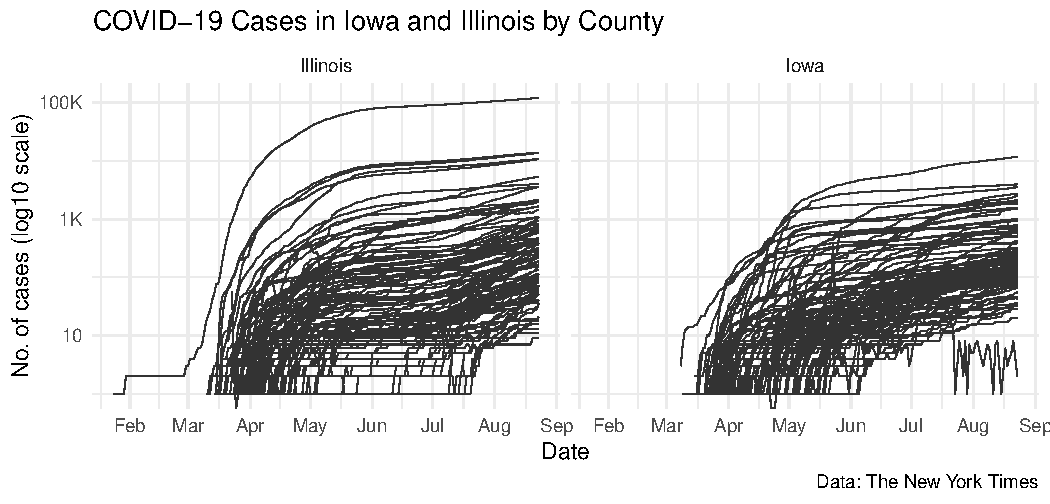
\includegraphics[width=\maxwidth]{figure/nytcases-1} 

}


\end{knitrout}
	
\end{frame}




\begin{frame}[fragile]{County level cases for Iowa and Illinois - per capita}
	
\begin{knitrout}\tiny
\definecolor{shadecolor}{rgb}{0.969, 0.969, 0.969}\color{fgcolor}\begin{kframe}
\begin{alltt}
\hlkwd{ggplot}\hlstd{(}\hlkwc{data} \hlstd{= county_level,} \hlkwc{mapping} \hlstd{=} \hlkwd{aes}\hlstd{(}\hlkwc{x} \hlstd{= date,} \hlkwc{y} \hlstd{= cases.per.10k,} \hlkwc{group} \hlstd{= county))} \hlopt{+}
  \hlkwd{geom_line}\hlstd{(}\hlkwc{size} \hlstd{=} \hlnum{0.25}\hlstd{,} \hlkwc{color} \hlstd{=} \hlstr{"gray20"}\hlstd{)} \hlopt{+}
  \hlkwd{scale_x_date}\hlstd{(}\hlkwc{date_breaks} \hlstd{=} \hlstr{"1 month"}\hlstd{,} \hlkwc{date_labels} \hlstd{=} \hlstr{"%b"}\hlstd{)}\hlopt{+}
  \hlkwd{scale_y_continuous}\hlstd{(}\hlkwc{labels} \hlstd{= scales}\hlopt{::}\hlkwd{label_number_si}\hlstd{())} \hlopt{+}
  \hlkwd{guides}\hlstd{(}\hlkwc{color} \hlstd{=} \hlnum{FALSE}\hlstd{)} \hlopt{+} \hlkwd{facet_wrap}\hlstd{(}\hlopt{~} \hlstd{state,} \hlkwc{ncol} \hlstd{=} \hlnum{2}\hlstd{)} \hlopt{+}
  \hlkwd{labs}\hlstd{(}\hlkwc{title} \hlstd{=} \hlstr{"COVID-19 Cases in Iowa and Illinois by County"}\hlstd{,}
       \hlkwc{x} \hlstd{=} \hlstr{"Date"}\hlstd{,} \hlkwc{y} \hlstd{=} \hlstr{"No. of cases per 10 000"}\hlstd{,} \hlkwc{caption} \hlstd{=} \hlstr{"Data: The New York Times"}\hlstd{)} \hlopt{+}
  \hlkwd{theme_minimal}\hlstd{()}
\end{alltt}
\end{kframe}

{\centering 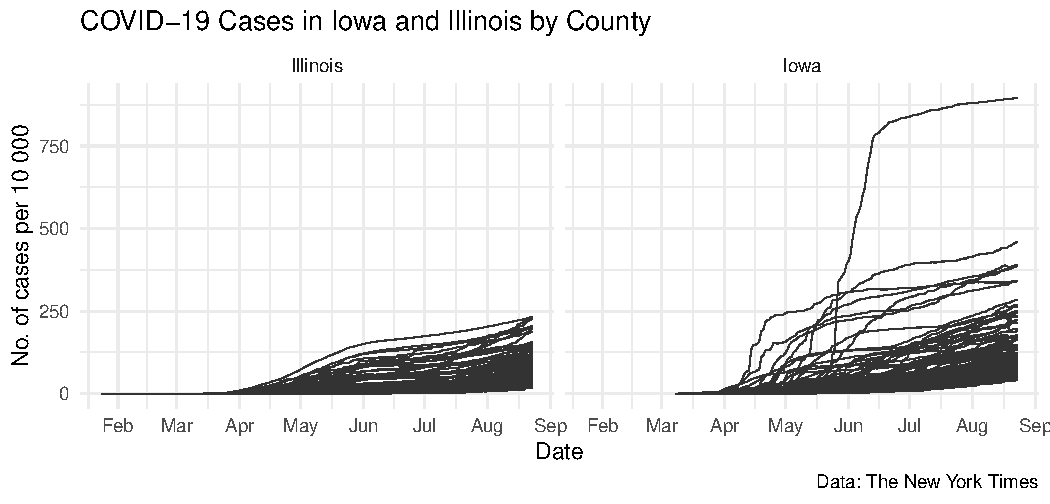
\includegraphics[width=\maxwidth]{figure/nytcapita-1} 

}


\end{knitrout}
	
\end{frame}



\begin{frame}[fragile]{State level cases for Iowa and Illinois - per capita}
	
\begin{knitrout}\tiny
\definecolor{shadecolor}{rgb}{0.969, 0.969, 0.969}\color{fgcolor}\begin{kframe}
\begin{alltt}
\hlkwd{ggplot}\hlstd{(}\hlkwc{data} \hlstd{= state_level,} \hlkwc{mapping} \hlstd{=} \hlkwd{aes}\hlstd{(}\hlkwc{x} \hlstd{= date,} \hlkwc{y} \hlstd{= cases.per.10k,} \hlkwc{color} \hlstd{= state))} \hlopt{+}
  \hlkwd{geom_line}\hlstd{(}\hlkwc{size} \hlstd{=} \hlnum{1}\hlstd{)} \hlopt{+}
  \hlkwd{scale_x_date}\hlstd{(}\hlkwc{date_breaks} \hlstd{=} \hlstr{"1 month"}\hlstd{,} \hlkwc{date_labels} \hlstd{=} \hlstr{"%b"}\hlstd{)}\hlopt{+}
  \hlkwd{scale_y_continuous}\hlstd{(}\hlkwc{labels} \hlstd{= scales}\hlopt{::}\hlkwd{label_number_si}\hlstd{())} \hlopt{+}
  \hlkwd{labs}\hlstd{(}\hlkwc{title} \hlstd{=} \hlstr{"COVID-19 Cases in Iowa and Illinois"}\hlstd{,}
       \hlkwc{subtitle} \hlstd{=} \hlstr{"Cases since March 15, 2020"}\hlstd{,}
       \hlkwc{x} \hlstd{=} \hlstr{"Date"}\hlstd{,} \hlkwc{y} \hlstd{=} \hlstr{"No. of cases per 10 000"}\hlstd{,} \hlkwc{caption} \hlstd{=} \hlstr{"Data: The New York Times"}\hlstd{)} \hlopt{+}
  \hlkwd{theme_minimal}\hlstd{()}
\end{alltt}
\end{kframe}

{\centering 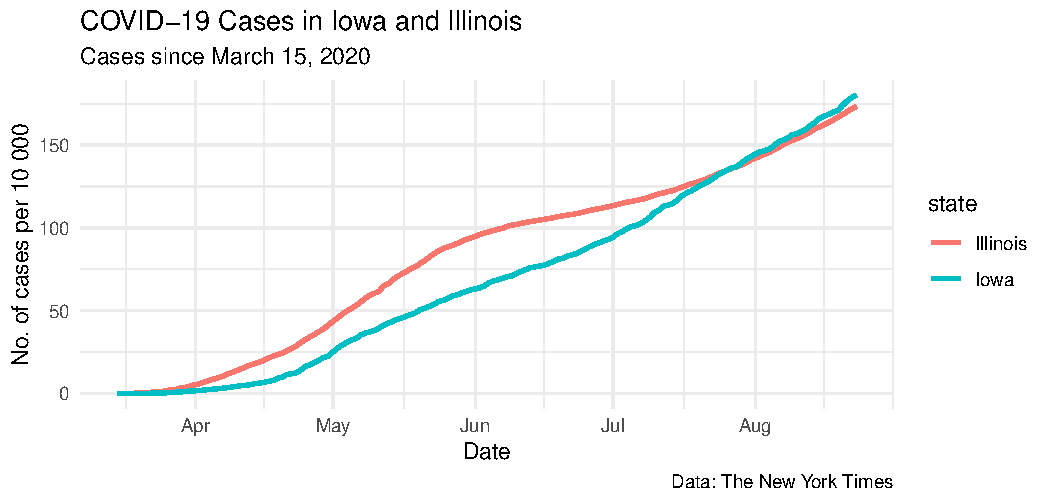
\includegraphics[width=\maxwidth]{figure/nytcapitastate-1} 

}


\end{knitrout}
	
\end{frame}


\begin{frame}[fragile]{Are the findings in the paper reproducible?}
	
\begin{knitrout}\tiny
\definecolor{shadecolor}{rgb}{0.969, 0.969, 0.969}\color{fgcolor}\begin{kframe}
\begin{alltt}
\hlstd{fit3} \hlkwb{<-} \hlkwd{glm}\hlstd{(cases.per.10k} \hlopt{~} \hlstd{state}\hlopt{*}\hlstd{time,} \hlkwc{data} \hlstd{= state_level)}
\hlkwd{summary}\hlstd{(fit3)}
\end{alltt}
\begin{verbatim}
## 
## Coefficients:
##                  Estimate Std. Error t value Pr(>|t|)    
## (Intercept)    -142.10981    9.86847 -14.400  < 2e-16 ***
## stateIowa       -13.71844   13.95612  -0.983    0.326    
## time              2.69285    0.03190  84.404  < 2e-16 ***
## stateIowa:time    0.33126    0.04512   7.342 4.17e-13 ***
## ---
## Signif. codes:  0 '***' 0.001 '**' 0.01 '*' 0.05 '.' 0.1 ' ' 1
## 
## (Dispersion parameter for gaussian family taken to be 12988.97)
## 
##     Null deviance: 224587838  on 1069  degrees of freedom
## Residual deviance:  13846245  on 1066  degrees of freedom
## AIC: 13177
## 
## Number of Fisher Scoring iterations: 2
\end{verbatim}
\end{kframe}
\end{knitrout}
	
\end{frame}


\begin{frame}[fragile]{Model-based predictions}
	
\begin{knitrout}\tiny
\definecolor{shadecolor}{rgb}{0.969, 0.969, 0.969}\color{fgcolor}\begin{kframe}
\begin{alltt}
\hlkwd{library}\hlstd{(ggeffects)}
\hlstd{ggeffects}\hlopt{::}\hlkwd{ggpredict}\hlstd{(fit3,} \hlkwc{terms} \hlstd{=} \hlstr{"state"}\hlstd{)} \hlopt
  \hlkwd{plot}\hlstd{()}
\end{alltt}
\end{kframe}

{\centering 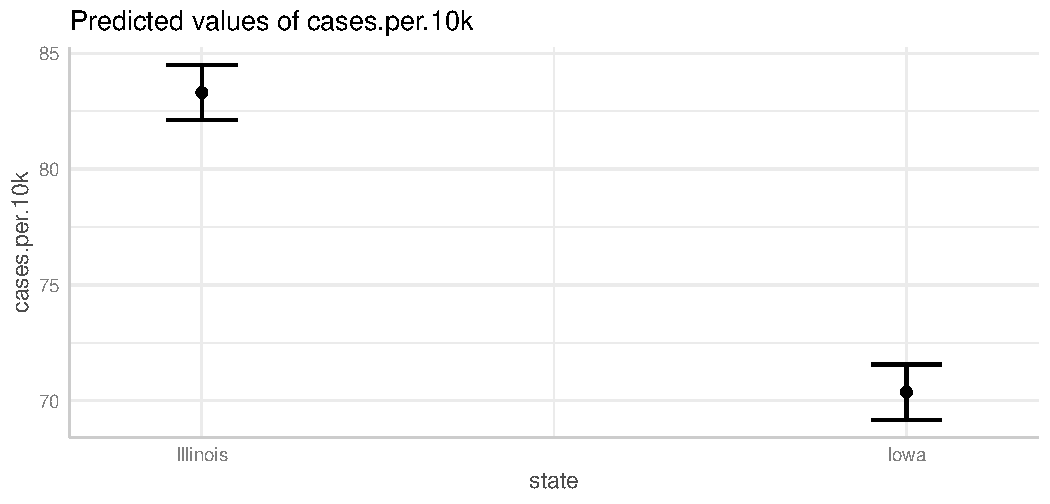
\includegraphics[width=\maxwidth]{figure/nytcapitastatemodel2-1} 

}


\end{knitrout}
	
\end{frame}


%\begin{frame}[allowframebreaks]
%\nocite{breiman1984classification}
%	\nocite{friedman2001elements}
%	\nocite{james2013introduction}
%	\nocite{lopez2015arbres}
%	\frametitle{References}
%\printbibliography
%\end{frame}


\begin{frame}[fragile]{Session Info}
	\tiny
	
\begin{knitrout}\tiny
\definecolor{shadecolor}{rgb}{0.969, 0.969, 0.969}\color{fgcolor}\begin{kframe}
\begin{verbatim}
R version 4.0.2 (2020-06-22)
Platform: x86_64-pc-linux-gnu (64-bit)
Running under: Pop!_OS 20.10

Matrix products: default
BLAS:   /usr/lib/x86_64-linux-gnu/openblas-pthread/libblas.so.3
LAPACK: /usr/lib/x86_64-linux-gnu/openblas-pthread/libopenblasp-r0.3.10.so

attached base packages:
[1] tools     stats     graphics  grDevices utils     datasets  methods  
[8] base     

other attached packages:
 [1] ggeffects_0.16.0    covdata_0.8         openintro_2.0.0    
 [4] usdata_0.1.0        cherryblossom_0.1.0 airports_0.1.0     
 [7] here_0.1            oibiostat_0.2.0     NCStats_0.4.7      
[10] FSA_0.8.30          forcats_0.5.1       stringr_1.4.0      
[13] dplyr_1.0.7         purrr_0.3.4         readr_1.4.0        
[16] tidyr_1.1.3         tibble_3.1.3        ggplot2_3.3.5      
[19] tidyverse_1.3.0     knitr_1.33         

loaded via a namespace (and not attached):
  [1] minqa_1.2.4        TH.data_1.0-10     colorspace_2.0-2  
  [4] ellipsis_0.3.2     rio_0.5.16         leaflet_2.0.3     
  [7] sjlabelled_1.1.7   rprojroot_2.0.2    snakecase_0.11.0  
 [10] estimability_1.3   ggstance_0.3.4     parameters_0.8.6  
 [13] ggdendro_0.1.22    fs_1.5.0           rstudioapi_0.13   
 [16] farver_2.1.0       ggrepel_0.8.2      mvtnorm_1.1-1     
 [19] fansi_0.5.0        lubridate_1.7.9    xml2_1.3.2        
 [22] codetools_0.2-16   mosaic_1.7.0       splines_4.0.2     
 [25] sjmisc_2.8.5       polyclip_1.10-0    jsonlite_1.7.2    
 [28] nloptr_1.2.2.2     broom_0.7.2        dbplyr_1.4.4      
 [31] ggforce_0.3.2      effectsize_0.3.3   compiler_4.0.2    
 [34] httr_1.4.2         sjstats_0.18.0     emmeans_1.5.1     
 [37] backports_1.2.1    assertthat_0.2.1   Matrix_1.2-18     
 [40] cli_3.0.1          formatR_1.8        tweenr_1.0.1      
 [43] htmltools_0.5.1.1  coda_0.19-4        gtable_0.3.0      
 [46] glue_1.4.2         Rcpp_1.0.7         carData_3.0-4     
 [49] cellranger_1.1.0   vctrs_0.3.8        sjPlot_2.8.5      
 [52] nlme_3.1-149       crosstalk_1.1.1    insight_0.9.6     
 [55] xfun_0.25          lme4_1.1-23        openxlsx_4.1.5    
 [58] rvest_1.0.0        lifecycle_1.0.0    mosaicCore_0.8.0  
 [61] pacman_0.5.1       statmod_1.4.34     zoo_1.8-8         
 [64] MASS_7.3-53        scales_1.1.1       hms_1.0.0         
 [67] sandwich_2.5-1     curl_4.3.2         mosaicData_0.20.1 
 [70] gridExtra_2.3      TeachingDemos_2.12 stringi_1.7.3     
 [73] highr_0.9          bayestestR_0.7.2   boot_1.3-25       
 [76] zip_2.2.0          rlang_0.4.11       pkgconfig_2.0.3   
 [79] evaluate_0.14      lattice_0.20-41    htmlwidgets_1.5.3 
 [82] labeling_0.4.2     tidyselect_1.1.1   ggformula_0.9.4   
 [85] plyr_1.8.6         magrittr_2.0.1     R6_2.5.1          
 [88] generics_0.1.0     multcomp_1.4-13    DBI_1.1.1         
 [91] pillar_1.6.2       haven_2.3.1        foreign_0.8-80    
 [94] withr_2.4.2        survival_3.2-3     abind_1.4-5       
 [97] performance_0.5.0  modelr_0.1.8       crayon_1.4.1      
[100] car_3.0-9          utf8_1.2.2         grid_4.0.2        
[103] readxl_1.3.1       data.table_1.14.0  blob_1.2.1        
[106] reprex_0.3.0       digest_0.6.27      xtable_1.8-4      
[109] munsell_0.5.0     
\end{verbatim}
\end{kframe}
\end{knitrout}
	
\end{frame}

\end{document}
